\documentclass[11pt,a4paper]{article}
\usepackage[utf8]{inputenc}
\usepackage[T1]{fontenc}
\usepackage{lmodern}
\usepackage{microtype}
\usepackage[margin=1in]{geometry}
\usepackage{amsmath,amssymb,amsthm}
\usepackage{booktabs}
\usepackage{array}
\usepackage{enumitem}
\usepackage{xcolor}
\usepackage{tikz}
\usetikzlibrary{arrows.meta,calc,positioning}
\usepackage{pgfplots}
\pgfplotsset{compat=1.17}
\setlength{\emergencystretch}{1.5em}
\usepackage[labelfont=bf,font=small,labelsep=period]{caption}
\usepackage[most]{tcolorbox}
\usepackage{needspace}
\usepackage{placeins}
\tcbset{paperbox/.style={breakable, enhanced, colback=gray!4, colframe=gray!55, boxrule=0.5pt, arc=2pt, left=6pt, right=6pt, top=5pt, bottom=5pt, fonttitle=\bfseries, coltitle=black, colbacktitle=gray!15, attach boxed title to top left={yshift=-2mm, xshift=4mm}, boxed title style={boxrule=0.5pt, colframe=gray!55}}}
\usepackage[colorlinks=true,linkcolor=blue!50!black,citecolor=blue!50!black,urlcolor=blue!50!black]{hyperref}

\theoremstyle{plain}
\newtheorem{theorem}{Theorem}
\newtheorem*{theorem2p}{Theorem 2$'$}
\newtheorem*{theorem4p}{Theorem 4$'$}
\theoremstyle{definition}
\newtheorem*{axiom}{Axiom}
\theoremstyle{remark}
\newtheorem*{remark}{Remark}

\newcommand{\tr}{\operatorname{tr}}
\newcommand{\E}{\mathbb{E}}
\newcommand{\R}{\mathbb{R}}
\newcommand{\C}{\mathbb{C}}
\newcommand{\RP}{\mathbb{RP}}
\newcommand{\CP}{\mathbb{CP}}
\newcommand{\SO}{\mathrm{SO}}
\newcommand{\SU}{\mathrm{SU}}
\newcommand{\PU}{\mathrm{PU}}
\newcommand{\PSp}{\mathrm{PSp}}
\newcommand{\PSO}{\mathrm{PSO}}
\newcommand{\Sp}{\mathrm{Sp}}
\newcommand{\U}{\mathrm{U}}
\newcommand{\adj}{\mathrm{adj}}
\newcommand{\Sym}{\mathrm{Sym}}
\newcommand{\diag}{\operatorname{diag}}

\title{An Operational Representation of Systems:\\ A Worked Construction in Lattice Gauge Theory}
\author{Edward Chalk\\ \small Sapientronic \quad \href{mailto:edward.chalk@sapientronic.ai}{edward.chalk@sapientronic.ai}}
\date{19 October 2026}

\begin{document}
\maketitle

\begin{abstract}
This paper introduces a minimal, ordinal representation of systems and tests it in lattice gauge theory. The representation takes a system to be three things: something that drives it, something that constrains it, and the system's own way of holding the two together. In a reservoir the water presses and the dam wall holds, and whether the whole leaks, bursts or stands is decided by neither on its own; it is the system's own conduct. The representation is minimal because it uses only those three roles.

The smallest part of a system, which we call an element, divides what reaches it between what it passes on and what it holds back. Only those two shares can be observed, and the representation is ordinal because it carries nothing but shares of a unit, and no absolute scale. The axes against which they are measured cannot, and each element has axes of its own, so a rule for carrying a state from one element to the next has to be supplied.

That is also the shape of lattice gauge theory: sites whose local frames no measurement can see, links that carry a rule between neighbouring frames, and observables that survive being carried round closed loops. The paper states the systems representation as axioms and shows that the theory's structures follow from them and from assumptions that are named: that relations act transitively, that amplitudes are real or complex, and a chosen form of the dynamics and of the loss round a loop. The rule on a link is an element of a group; that the relations form a group is one of the axioms, and which group it can be is then derived. The invisibility of frames is the gauge freedom, and it gives Gauss's law. The loss of carrying a state round a loop, averaged over the state, is the Wilson action, and whether the amplitudes are real or complex, and which group acts, fixes the representation it is written in. Keeping the states as variables fixes an interaction between neighbouring loops, which is checked by direct diagonalisation.

The aim is to show that a representation of systems in general can be made precise enough to construct and check definite structure in an exacting theory, and that the theory then becomes intelligible as the consequence of a few statements about systems. The paper does not derive the continuum theory and says nothing about the mass gap.
\end{abstract}

\noindent\small Every computation referred to is reproduced by the accompanying code (\texttt{minos\_yang\_mills.py}, with its output beside it), which travels with the paper and is archived at \href{https://doi.org/10.5281/zenodo.23454340}{doi:10.5281/zenodo.23454340}.

\noindent\copyright\ 2026 Edward Chalk. All rights reserved.
\normalsize

\clearpage
\section{The problem, and the purpose of the paper}

\subsection{A representation of systems, tested in lattice gauge theory}

This paper introduces a minimal, ordinal representation of systems, which we call MINOS, and tests it in lattice gauge theory. Minimal, because it is built from the fewest roles under which something is a system at all. Ordinal, because it carries no absolute magnitudes, only shares of a unit that each element sets for itself.

\S\ref{sec:notions} says what it is, why it bears on lattice gauge theory, and why it may be a sensible way of thinking about that theory. The sections after it make each statement precise and test it.

\subsection{Can a representation of systems be made precise enough for mathematical physics?}

The question is whether a representation built to describe systems in general can be stated precisely enough for mathematical physics to work with; whether, carried into lattice gauge theory, it produces structure that is definite and calculable; and whether that structure stands up to stated assumptions, proofs, and checks that can fail. Lattice gauge theory is a demanding test because its symmetry structure and its finite-graph formulation are mathematically explicit: a finite graph carries finitely many group-valued link variables, every statement about them can be made exact, and an incorrect step can be exposed by explicit calculation or counterexample.

\subsection{The paper tests the representation and uses it to make the theory intelligible}

The paper has two purposes, and neither is a claim about nature. The first is to test the representation: to see whether it can be stated as axioms, applied without renaming anything, made to produce consequences that can be computed and checked, and corrected where it is wrong. We call this the \textbf{methodological} purpose. The second is to make lattice gauge theory easier to understand. Gauge covariance, Gauss's law, the choice of representation in the action and the Casimir kinetic term each come out as consequences of a few statements about systems in general, so that someone who understands systems can see why the theory has the shape it has, and someone who understands the theory can see what a systems account adds and what it only restates. We call this the \textbf{explanatory} purpose. In short, the aim is to show that \textbf{the representation admits precise mathematical formulation and testing}. Nothing here is a prediction, and nothing here is offered as the only possible representation of systems. It is one proposed representation, made precise, and put to a hard test.

\subsection{The representation holds up, with qualifications, and produces three results}

The answer we report is positive, with qualifications, and the qualifications are part of the method. Every step from the representation to a lattice structure either follows from the stated axioms or rests on a hypothesis we name. The hypotheses are few, and they are listed in \S\ref{sec:axioms}. The results are of three kinds: what is derived, what is reconstructed under assumptions, and what is a consequence of a specified model. The three are kept apart throughout, and \S\ref{sec:interp} says, for each result, which it is.

Three results carry the argument.
\begin{enumerate}[leftmargin=2em, itemsep=3pt]
\item \textbf{The readable geometry determines the action.} Under a stated return-loss rule, the readable state geometry determines the representation content of the lattice action, and determines it differently for real and for complex amplitudes (\S\ref{sec:central}). This shows that the representation makes a distinction with consequences for the action.
\item \textbf{The gauge geometry follows.} The same rule, with the relativity of frames and the group postulate A3, gives the permitted groups, the local freedom, Gauss's law, and the Casimir kinetic term through the invariant information metric (\S\S\ref{sec:geometry}--\ref{sec:central}). This shows that the representation organises known structure under stated assumptions.
\item \textbf{The pure theory is an averaged model, and the full model fixes an interaction.} The pure lattice gauge theory the construction yields is a model in which the loop's loss is defined as its average over the readable pole; equivalently, it is the leading term of a limit in which the poles' own stiffness grows. The full object is a gauge theory coupled to projective matter, the poles themselves. With the poles kept as dynamical variables, the same construction fixes a particular interaction between neighbouring plaquettes whose form is not a free choice (\S\ref{sec:consequence}). This shows that, once a model is specified, it determines quantities that can be calculated and checked.
\end{enumerate}
The analytical results and the specified numerical models are checked as described in \S\ref{sec:verification}, and the checks are supplied. Figure~\ref{fig:map} sets out the chain from the axioms to these results and marks where each assumption enters.

\begin{figure}[!htbp]
\centering
% Figure 5: the chain from the axioms to the results, with the kind of each result
\begin{tikzpicture}[>=Stealth, font=\footnotesize, node distance=4.5mm,
  stepbox/.style={draw, rounded corners=2pt, align=left, text width=9.1cm, inner sep=5pt},
  derived/.style={stepbox, fill=white},
  recon/.style={stepbox, fill=gray!12},
  model/.style={stepbox, fill=gray!28},
  uses/.style={anchor=east, align=right, text width=4.6cm, inner sep=2pt, font=\small\itshape},
  key/.style={draw, rounded corners=2pt, inner sep=3pt, font=\scriptsize, text width=2.7cm, align=center}]
\node[derived] (t1) {\textbf{Theorem 1.} A3 postulates that the relations between frames form a closed connected group $G$; the theorem constrains it: a subgroup of $\PU(N)$ ($\C$) or of $\SO(N)$ ($\R$), classified. Every element's frame may be changed independently: local gauge freedom, $U_{x\to y}\mapsto g_yU_{x\to y}g_x^{-1}$. \textbf{The fork:} nothing in A1--A6 selects real or complex.};
\node[derived, below=of t1] (lat) {\textbf{The construction (\S\ref{sec:construction}).} Configurations $G^E\times(\mathbb P^{N-1})^V$: relations on the interfaces, one held pole per element, drive poles transported by the interface rule. Readables: pass shares and junction angles. Gauss's law, with the pole's charge as its source.};
\node[derived, below=of lat] (meas) {\textbf{The invariant measure (\S\ref{sec:central}).} Round on $S^{N-1}$ for real amplitudes; Fubini--Study on $\CP^{N-1}$ for complex. They differ.};
\node[derived, below=of meas] (t2) {\textbf{Theorems 2, 2$'$.} The averaged return loss is a Wilson character action: the \textbf{$\SU(N)$ adjoint} on the complex branch (restricted on the symplectic alternative), \textbf{traceless symmetric} (spin two for $N=3$) on the real. The readable geometry determines the representation content.};
\node[derived, below=of t2] (t3) {\textbf{Theorem 3.} The information metric on relations is bi-invariant; its Laplacian is the quadratic Casimir.};
\node[recon, below=of t3] (t4) {\textbf{Theorem 4 (the averaged model).} $H=\frac{g^2}{2}\sum_\ell\Delta_\ell+\frac1{g^2}\sum_pc(U_p)$ on frame-invariant states: Kogut--Susskind in the adjoint (traceless symmetric) reading. The form is assumed, the content of each term forced.};
\node[model, below=of t4] (t4p) {\textbf{Theorem 4$'$ (the poles live).} There is no pole-neutral sector. With the poles dynamical at stiffness $\kappa$, the character action is the leading term and the next fixes a two-plaquette interaction $K$ wherever two paths are read through one element: its coefficients and angular dependence are not free. Free numbers: $g$ and $\kappa$.};
\foreach \a/\b in {t1/lat, lat/meas, meas/t2, t2/t3, t3/t4, t4/t4p} \draw[->, thick] (\a) -- (\b);
% what each step uses, on the left
\node[uses] at ($(t1.west)+(-0.3,0)$) {A1--A3b, A6; the interface rule of A4\\ (Wigner; Onishchik; Montgomery--Samelson, Borel)};
\node[uses] at ($(lat.west)+(-0.3,0)$) {A4: adjacency is assumed, not derived};
\node[uses] at ($(meas.west)+(-0.3,0)$) {A2, A3, A3b; \textbf{A1$\C$ is a hypothesis}};
\node[uses] at ($(t2.west)+(-0.3,0)$) {\textbf{H1}, the loss rule: one minus the returned share, averaged};
\node[uses] at ($(t3.west)+(-0.3,0)$) {A2, A3 (Helgason)};
\node[uses] at ($(t4.west)+(-0.3,0)$) {\textbf{A5}: kinetic plus potential, assumed; H1's average};
\node[uses] at ($(t4p.west)+(-0.3,0)$) {A4's mean over the path's elements; \textbf{the stiffness $\kappa$}, not fixed by the axioms};
% key
\node[key, fill=white, anchor=north west] (k1) at ($(t4p.south west)+(0,-0.45)$) {derived from the postulates};
\node[key, fill=gray!12, right=2mm of k1] (k2) {reconstructed under stated assumptions};
\node[key, fill=gray!28, right=2mm of k2] (k3) {consequence of the specified model};
\end{tikzpicture}

\caption{The chain from the axioms to the results. Each box names a result; the note to its left names what the result uses. The shading marks the three kinds of result of \S\ref{sec:interp}: derived from the representation's postulates, reconstructed under a stated assumption, or a consequence of the specified model.}
\label{fig:map}
\end{figure}

\subsection{The order of the sections}

The sections are these.
\begin{itemize}[leftmargin=2em, itemsep=1pt]
\item \S\ref{sec:notions} explains the notions in plain terms and says why they fit lattice gauge theory.
\item \S\ref{sec:primitive} states the primitive: the triad of drive, constraint and relation; the element as a binary comparison; and the rule that only shares can be read.
\item \S\ref{sec:axioms} states the axioms and marks each as a postulate of the representation or an assumption added for the domain.
\item \S\ref{sec:geometry} composes relations and obtains the gauge geometry: the group, the local freedom, the lattice construction with its poles, and Gauss's law.
\item \S\ref{sec:central} obtains the central result, that under the loss rule the readable geometry determines the representation content of the action, and from it the averaged Hamiltonian.
\item \S\ref{sec:consequence} keeps the poles live and obtains the interaction they induce.
\item \S\ref{sec:verification} lists the checks.
\item \S\ref{sec:interp} says what is derived, what is reconstructed, what is model-dependent, and what is open.
\end{itemize}

\subsection{Nothing is claimed about Yang--Mills itself, the continuum limit, or the mass gap}

The paper does not claim the following.
\begin{itemize}[leftmargin=2em, itemsep=1pt]
\item It does not derive Yang--Mills theory from the bare notion of a system. Complex amplitudes are a hypothesis; so is the kinetic-plus-potential form of the dynamics; so is the loss functional.
\item It makes no statement about the continuum limit or the mass gap.
\item It does not claim that the representation theory it uses---character decompositions, invariant integration, degenerate perturbation theory---is new.
\item It leaves open the general composition law for independently specified systems, which is where the representation's own content would next be tested.
\end{itemize}

\clearpage
\section{The notions, and why they fit the subject}\label{sec:notions}

The notions the paper is built from are explained here in plain terms, with the reasons they are a sensible way to think about lattice gauge theory. \S\ref{sec:primitive} and \S\ref{sec:axioms} state the same things precisely; the rest of the paper tests them.

\subsection{A system: drive, constraint, relation}

Take anything one would ordinarily call a system: a reservoir with its dam, a valve, a market, a cell. In each there is something that drives it, something that constrains it, and a conduct that results (Figure~\ref{fig:system}a). In the reservoir the water presses. The dam wall holds. Whether the whole leaks, bursts or stands is settled by neither the water alone nor the wall alone; it is settled by the system the two make up, the reservoir and its dam together. We call the three roles the \emph{drive}, the \emph{constraint} and the \emph{relation}. The relation is the system's own contribution: how a given drive and a given constraint cohere into conduct. The representation uses these three roles and nothing else, and for that reason we call it \emph{minimal}.

The roles are not things. The water that drives the wall is what the river above is constrained to deliver, and what is constraint to one part of a system is drive to the next. The names belong to where one stands when one reads the system, and the representation keeps only the names. That is what lets it be a representation of systems in general rather than of dams: it never says what the drive is made of, only that there is one.

\subsection{The element: one angle, two shares}

The smallest thing a system can do with a drive and a constraint is to divide what reaches it: so much passed on, so much held (Figure~\ref{fig:system}b). If the two shares add up to the whole, the division is a single angle. The share passed is the square of the cosine of the angle, the share held is the square of the sine, and the two sum to one. We call such a divider an \emph{element}. A reservoir with its dam is an element: of the water that arrives, so much goes through and so much is held back. A valve is an element, and so is a membrane. A system with several inlets and outlets is several elements, one for each interface, and is assembled from them. The angle is the whole of the element's state. There is no further number in it, and in particular there is no size. The element divides its own unit, and the unit is whatever reaches it. The two extremes of the angle are states of the element. At one everything is passed and nothing held, an open conduit; at the other everything is held and nothing passed, a closed valve. Both are still elements, because the other pole is still there, pressing or bounding. What is not an element is a unit with one pole only, and the next subsection says why.

\begin{figure}[!htbp]
\centering
% Figure: what a system is in the representation — the dam, and the element as a divider
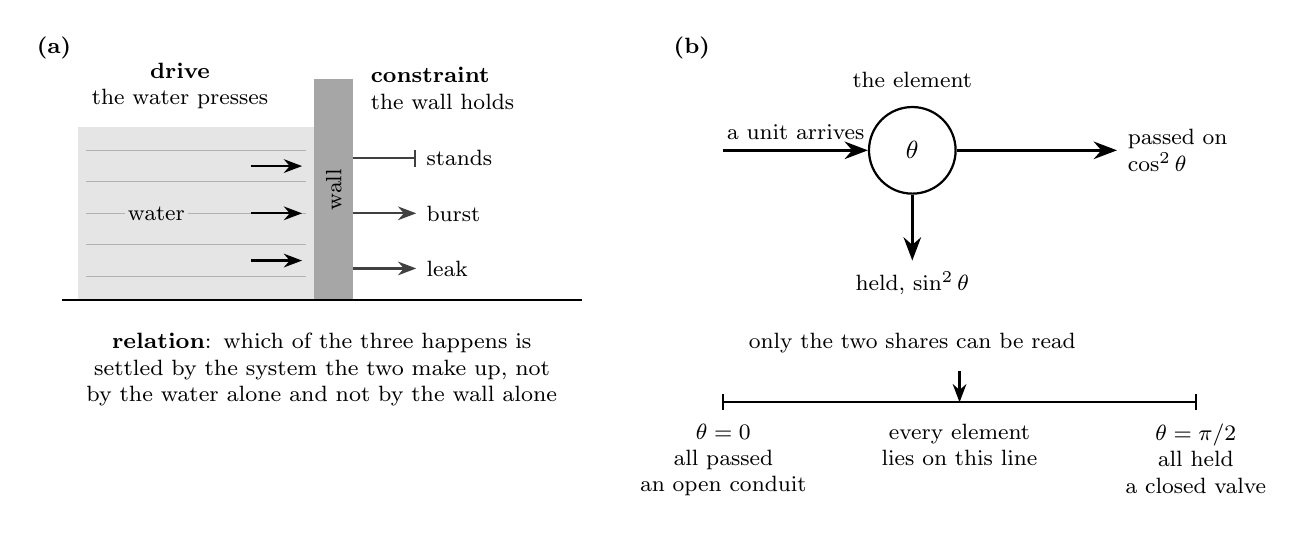
\begin{tikzpicture}[>=Stealth, font=\small]
% ---------------- (a) the dam: drive, constraint, and the system's own conduct ----------------
\begin{scope}
  \node[font=\footnotesize\bfseries] at (-0.3,3.2) {(a)};
  % water
  \fill[gray!20] (0,0) rectangle (3,2.2);
  \foreach \y in {0.3,0.7,...,2.0} \draw[gray!60] (0.1,\y) -- (2.9,\y);
  \node[font=\footnotesize, align=center, fill=gray!20, inner sep=1pt] at (1.0,1.1) {water};
  % wall
  \fill[gray!70] (3,0) rectangle (3.5,2.8);
  \node[font=\footnotesize, rotate=90] at (3.25,1.4) {wall};
  % ground
  \draw[thick] (-0.2,0) -- (6.4,0);
  % the drive: pressure arrows
  \foreach \y in {0.5,1.1,1.7} \draw[->, thick] (2.2,\y) -- (2.85,\y);
  \node[font=\footnotesize, align=center, anchor=south] at (1.3,2.3) {\textbf{drive}\\ the water presses};
  \node[font=\footnotesize, align=left, anchor=south west] at (3.6,2.3) {\textbf{constraint}\\ the wall holds};
  % the conduct: three possibilities on the dry side
  \draw[->, thick, gray!50!black] (3.5,0.4) -- (4.3,0.4) node[right, font=\footnotesize, black] {leak};
  \draw[->, thick, gray!50!black] (3.5,1.1) -- (4.3,1.1) node[right, font=\footnotesize, black] {burst};
  \draw[-|, thick, gray!50!black] (3.5,1.8) -- (4.3,1.8) node[right, font=\footnotesize, black] {stands};
  \node[font=\footnotesize, align=center, text width=6.4cm, anchor=north] at (3.1,-0.3) {\textbf{relation}: which of the three happens is settled by the system the two make up, not by the water alone and not by the wall alone};
\end{scope}
% ---------------- (b) the element as a divider ----------------
\begin{scope}[xshift=8.4cm]
  \node[font=\footnotesize\bfseries] at (-0.6,3.2) {(b)};
  \node[draw, thick, circle, minimum size=1.1cm, inner sep=0pt] (e) at (2.2,1.9) {$\theta$};
  \node[font=\footnotesize] at (2.2,2.8) {the element};
  \draw[->, very thick] (-0.2,1.9) -- (e) node[midway, above, font=\footnotesize] {a unit arrives};
  \draw[->, very thick] (e) -- (4.8,1.9) node[right, font=\footnotesize, align=left] {passed on\\ $\cos^2\theta$};
  \draw[->, very thick] (e) -- (2.2,0.5) node[below, font=\footnotesize, align=center] {held, $\sin^2\theta$};
  \node[font=\footnotesize, align=center, anchor=north] at (2.2,-0.3) {only the two shares can be read};
  % the dial of theta
  \draw[thick] (-0.2,-1.3) -- (5.8,-1.3);
  \foreach \x in {-0.2,5.8} \draw[thick] (\x,-1.4) -- (\x,-1.2);
  \draw[->, thick] (2.8,-0.9) -- (2.8,-1.3);
  \node[font=\footnotesize, align=center, anchor=north] at (-0.2,-1.45) {$\theta=0$\\ all passed\\ an open conduit};
  \node[font=\footnotesize, align=center, anchor=north] at (5.8,-1.45) {$\theta=\pi/2$\\ all held\\ a closed valve};
  \node[font=\footnotesize, align=center, anchor=north] at (2.8,-1.45) {every element\\ lies on this line};
\end{scope}
\end{tikzpicture}

\caption{What a system is in the representation. (a) A reservoir and its dam: the water drives, the wall constrains, and which conduct results is the contribution of the system the two make up, the relation. (b) The element: a unit arrives and is divided between what is passed on and what is held. The division is one angle. Its two extremes, all passed and all held, are states of the element; a unit with one pole only has no angle. Only the two shares can be read.}
\label{fig:system}
\end{figure}

\subsection{A system exists only while both opposites are present}

The two ends of the element are where the representation's notion of a system shows most plainly. A drive and a constraint are opposed tendencies. Left to itself the first passes everything and the second holds everything. A system is neither of them prevailing. It is the two held against each other, and it exists only while they are. Remove the constraint and the drive runs on without bound: the system has not become a freer system, it has ceased to be one. Remove the drive and the constraint holds and passes nothing: the system has not become a steadier one, it has ceased to be one. The two failures are a burst and a death, and between them lies every system that works. The opposites, then, are not two constituents. They are one system in its two manners, and the element of \S\ref{sec:comparison} is the measure of how far it inclines to either. That is what the minimality of the triad amounts to. A system is the holding-together of opposites, and what holds none together is not a system.

This line of thought can be traced back to Heraclitus, one of the earliest Greek philosophers, who taught at Ephesus around the end of the sixth century BC. He saw that a thing can be held together by the very tension that seems to divide it, and his example was the bow and the lyre. In his words, people do not understand how what is at variance with itself agrees with itself; there is a connection that is stretched back on itself, as in the bow and the lyre (fragment 22~B51 in the Diels--Kranz numbering \cite{krs}). A bow is a bow only while the stave and the string pull against each other. Slacken either and you are left with a stick and a cord. That is a system in exactly the sense set out above: two opposed tendencies, and a thing that exists only while both are present. In another fragment (B60) he says that the way up and the way down are one and the same. The road does not have an identity apart from its two directions; it is one road because it carries both. That is the point about identity made above. A system is not a thing that happens to have a drive and a constraint. It has an identity of its own only because it contains the two opposites, and when either goes the system goes with it. The fragments are cited for that idea; the argument of the paper starts from the axioms of \S\ref{sec:axioms}.

\subsection{What can be read: shares, not frames}

The representation makes one rule about evidence. Of an element, only the two shares can be observed. Consider what a measurement on the reservoir and its dam can yield: how much passed, and how much was held. It cannot yield the sign of the angle, because an angle of $\theta$ and an angle of $-\theta$ divide the unit in the same way. It cannot yield the orientation of the pair of axes against which the angle is measured, which we call the element's \emph{frame}, because turning the axes together with the state turns nothing that can be observed. And it cannot yield any phase the angle might carry. We say that only shares are \emph{readable}.

This is the representation's rule, axiom A2 of \S\ref{sec:axioms}, and it is a postulate: it is not claimed that every measurement of every system returns only a share. It is modelled on the one kind of measurement that does. A comparison of a state with an outcome yields how much of the state lies along the outcome, and nothing else. Everything else one might say about the state is a description of it in some frame, and a frame is a choice, not a datum. Because an element carries only shares of its own unit, and no absolute magnitude, we call the representation \emph{ordinal} rather than metric. The word is not used in the statistician's strict sense. A share is a number, and the paper computes with it. What the representation lacks is a scale: a share of a quarter says what fraction of the element's unit was passed, and nothing about how large the unit is. If a system is to have a size, the size has to be built up from the way its elements are put together. In a theory whose only scale is self-generated, that is the right place to start.

\subsection{Frames, and the relation between them}

Each element's angle is measured in a frame of its own, its own pair of axes, and no observation sees that frame. Two elements therefore have two frames, and nothing in either element says how the one is set against the other. To carry the state of one element into the frame of the next, so that the next can divide it in its turn, a rule for the carrying is needed. That rule is the \emph{relation} between the two frames. It is not derived from the elements, because the elements do not contain it. It is supplied, which is what the triad said of the relation from the start: it is the part of the system that is in neither pole.

Supplied relations can be chained. Carry a state from one element to the next, and to the next, and round again to the first. Nothing guarantees that it comes back as it left. Whether it does is readable, because it is a share: how much of the state, carried round, still lies along the state it started as. That returning share is the one thing a closed chain of relations lets anyone read, and the paper's central result is about what it costs.

\subsection{Lattice gauge theory in the same terms}

Lattice gauge theory is the standard way of putting a gauge theory, such as the theory of the strong interaction, on a finite grid so that it can be computed. Only its shape is needed here. The theory lives on a lattice of sites joined by links. Each site carries a frame of its own, a choice of axes for the quantities defined there, and the central fact of a gauge theory is that this choice is invisible: one may change the frame at every site independently, and no observable quantity changes. Each link carries a rule, an element of a symmetry group, for carrying a quantity from the frame at one end to the frame at the other. In the pure theory, what can be observed is what is left when a quantity is carried round a closed loop of links and compared with itself; when matter sits at the sites, there are also gauge-invariant quantities on single links, formed from the matter at the two ends. The theory's action is built from the smallest such loops, and Gauss's law is the statement that physical states do not depend on the choice of frames.

Figure~\ref{fig:correspondence} sets the two descriptions side by side. An element with a frame of its own that no observation can see is a site. The relation that must be supplied between two elements' frames is a link. The rule that only shares are readable is the rule that only gauge-invariant quantities are observable. The loss of carrying an element's state round a closed path and comparing it with itself is the action on a loop. The match is more than one of vocabulary. A gauge theory is, by definition, a theory in which a local choice of frame is unobservable and in which what is observable is what survives being carried round a loop. Those are the two statements the representation makes about any system: that an element's frame is its own and cannot be read, and that only shares can be read, including the share that returns from a closed chain. A representation of systems without those two features would not fit a gauge theory. This one has them because it was built from what can be read of a system at all, and a gauge theory is the physics of exactly that restriction.

The correspondence is not used as an analogy. In this paper the systems statements come first, as axioms, and the theory's structures are shown to follow from them: which groups may sit on the links, given that the relations form one; the local freedom and the transformation law; Gauss's law; the representation in which the action is written; and the kinetic term.

\Needspace*{12\baselineskip}
\subsection{Why it may be a sensible way to think about the subject}

\begin{enumerate}[leftmargin=2em, itemsep=3pt]
\item \textbf{It explains structure that the theory otherwise takes as given.} Which group the link variable may lie in, that the frames are unobservable, that the action is a character of the loop: each is here a consequence of what any system must have, of what can be read of it, and of the postulate that the relations form a group.
\item \textbf{It makes a distinction the theory does not make by itself}, between what an element can read of its own state and what a probe with a frame of its own can read. The distinction has a consequence. The action an element reads is in the adjoint representation of the full unitary group, not the fundamental, and it is in a different representation again when the amplitudes are real rather than complex.
\item \textbf{It says what the pure gauge theory is an average over.} The element's own state, which the paper calls its pole, is averaged away in the pure theory. Kept, it is matter of a definite kind, and it induces an interaction between neighbouring loops whose form is fixed.
\item \textbf{Every step can fail.} Each is a theorem or a computation that can be checked, and all of them were run.
\end{enumerate}

\begin{figure}[!htbp]
\centering
% Figure: the systems representation and lattice gauge theory side by side
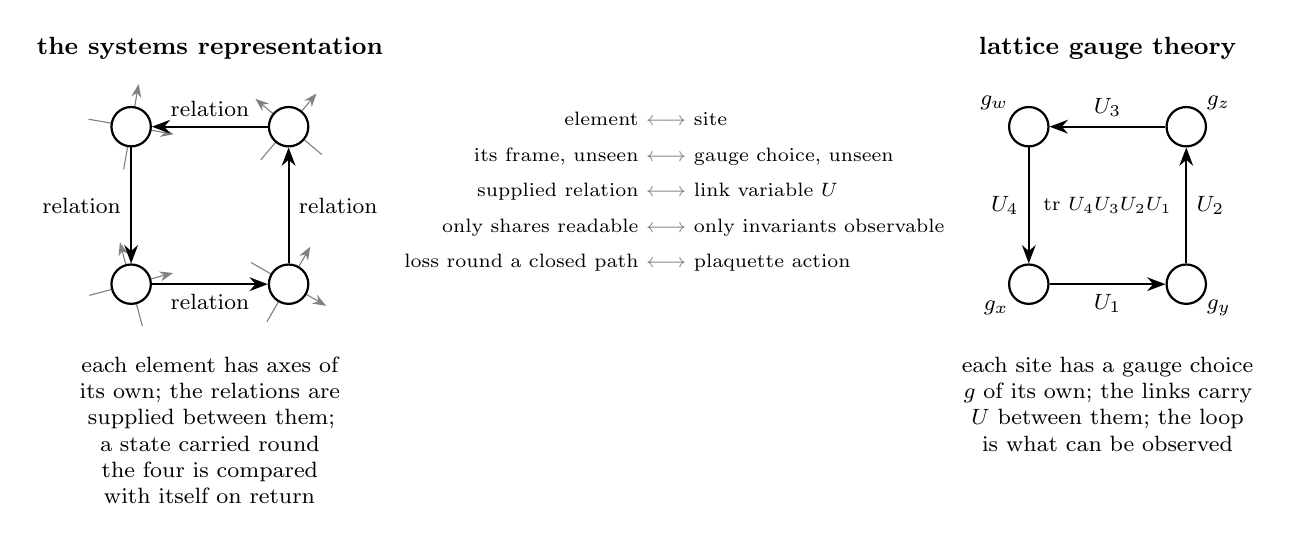
\begin{tikzpicture}[>=Stealth, font=\footnotesize,
  elem/.style={circle, draw, thick, fill=white, minimum size=5mm, inner sep=0pt},
  frame/.style={gray, ->, thin},
  row/.style={align=center, text width=5.2cm}]
% ---------------- left: the systems representation ----------------
\begin{scope}
  \node[font=\small\bfseries] at (1.0,3.0) {the systems representation};
  \foreach \x/\y/\r in {0/0/15, 2.0/0/-30, 2.0/2.0/50, 0/2.0/-10} {
    \begin{scope}[shift={(\x,\y)}, rotate=\r]
      \draw[frame] (-0.55,0) -- (0.55,0);
      \draw[frame] (0,-0.55) -- (0,0.55);
    \end{scope}
  }
  \foreach \n/\x/\y in {a/0/0, b/2.0/0, c/2.0/2.0, d/0/2.0} \node[elem] (\n) at (\x,\y) {};
  \draw[->, thick] (a) -- node[below] {relation} (b);
  \draw[->, thick] (b) -- node[right] {relation} (c);
  \draw[->, thick] (c) -- node[above] {relation} (d);
  \draw[->, thick] (d) -- node[left] {relation} (a);
  \node[anchor=north, align=center, text width=3.8cm] at (1.0,-0.8) {each element has axes of its own; the relations are supplied between them; a state carried round the four is compared with itself on return};
\end{scope}
% ---------------- right: lattice gauge theory ----------------
\begin{scope}[xshift=11.4cm]
  \node[font=\small\bfseries] at (1.0,3.0) {lattice gauge theory};
  \foreach \n/\x/\y in {A/0/0, B/2.0/0, C/2.0/2.0, D/0/2.0} \node[elem] (\n) at (\x,\y) {};
  \draw[->, thick] (A) -- node[below] {$U_1$} (B);
  \draw[->, thick] (B) -- node[right] {$U_2$} (C);
  \draw[->, thick] (C) -- node[above] {$U_3$} (D);
  \draw[->, thick] (D) -- node[left] {$U_4$} (A);
  \node[anchor=east, inner sep=1pt] at ($(A)+(-0.22,-0.3)$) {$g_x$};
  \node[anchor=west, inner sep=1pt] at ($(B)+(0.22,-0.3)$) {$g_y$};
  \node[anchor=west, inner sep=1pt] at ($(C)+(0.22,0.3)$) {$g_z$};
  \node[anchor=east, inner sep=1pt] at ($(D)+(-0.22,0.3)$) {$g_w$};
  \node[font=\scriptsize] at (1.0,1.0) {$\tr\,U_4U_3U_2U_1$};
  \node[anchor=north, align=center, text width=3.8cm] at (1.0,-0.8) {each site has a gauge choice $g$ of its own; the links carry $U$ between them; the loop is what can be observed};
\end{scope}
% ---------------- middle: the dictionary ----------------
\node[font=\scriptsize] at (6.9,1.2) {%
\renewcommand{\arraystretch}{1.6}%
\begin{tabular}{@{}r@{\ {\color{gray}$\longleftrightarrow$}\ }l@{}}
element & site\\
its frame, unseen & gauge choice, unseen\\
supplied relation & link variable $U$\\
only shares readable & only invariants observable\\
loss round a closed path & plaquette action
\end{tabular}};
\end{tikzpicture}

\caption{The two descriptions side by side. On the left, four elements, each with axes of its own, joined by supplied relations. On the right, four sites of a lattice, each with a gauge choice of its own, joined by link variables. The middle column is the dictionary. The paper does not use the dictionary as an analogy; it states the left-hand side as axioms and derives the right-hand side.}
\label{fig:correspondence}
\end{figure}

Table~\ref{tab:terms} collects the terms introduced in this section, with their counterparts in lattice gauge theory and the section in which each is made precise.

\begin{table}[!htbp]
\centering\small
\caption{The terms used in this paper, in plain words, with their lattice counterparts.}
\label{tab:terms}
\begin{tabular}{@{}>{\raggedright\arraybackslash}p{2.3cm}>{\raggedright\arraybackslash}p{6cm}>{\raggedright\arraybackslash}p{3.9cm}>{\raggedright\arraybackslash}p{1.9cm}@{}}
\toprule
term & meaning & in lattice gauge theory & made precise in\\
\midrule
drive, constraint & what moves a system and what holds it; the two \emph{poles} of an element & the two outcome axes of a comparison & \S\ref{sec:primitive}\\
relation & the system's own way of holding drive and constraint together; between two elements, the rule for carrying a state from one frame to the other & the link variable $U$ & \S\ref{sec:primitive}, \S\ref{sec:geometry}\\
element & the smallest part of a system: one angle dividing a unit into a passed share and a held share & a site, with its state & \S\ref{sec:comparison}\\
share & the passed or held fraction of the unit; the only thing that can be read & a gauge-invariant quantity & \S\ref{sec:comparison}\\
readable & determined by the shares against every measurement & observable & \S\ref{sec:axioms}, A2\\
frame & the axes an element's angle is measured against; unreadable; each element has its own & the local gauge choice at a site & \S\ref{sec:primitive}\\
pole (held, drive) & the element's own state; the state it receives along an interface & the matter field at a site & \S\ref{sec:construction}\\
loss round a path & one minus the share that returns when a state is carried round a closed path & the plaquette action & \S\ref{sec:central}\\
\bottomrule
\end{tabular}
\end{table}

\clearpage
\section{The primitive}\label{sec:primitive}

The notions of \S\ref{sec:notions}, stated in the form the rest of the paper uses.

\subsection{The triad: drive, constraint, relation}

A system, in this representation, has three roles (\S\ref{sec:notions}). Something \textbf{drives} it: a flow, a pressure, a demand, a field. Something \textbf{constrains} it: a bound, a rule, a conservation law, a capacity. How the two cohere into conduct is contained in neither and must be supplied; we call it the \textbf{relation}. Each is empty without the other two.

Three and not two, because a drive and a constraint do not determine what happens; the same pressure against the same wall gives a leak, a burst or a standing load, and what decides is a part of the system, not of its surroundings. Three and not four, because anything further one might name---a state, an output, a history---is a reading of these three or a composite of such triads. The claim of \emph{minimality} is this: the triad is the smallest set of roles under which the word \emph{system} applies, and the representation builds everything from the roles and nothing from their contents.\footnote{\emph{A note on the name.} The acronym was chosen for its words. The fit with the Minos of classical mythology is close enough to record and too slight to lean on. The king is remembered for his \textbf{law}, received and administered, and for his \textbf{royal will} and what its excesses cost him. The third thing remembered of him, that he judges the passage of the dead, is not a third attribute. It is what the meeting of the first two made of him: by his law a judge, by his will a man who had himself made the passage. The triad has the same form: a constraint, a drive, and a relation that is not a third ingredient but what their meeting supplies.}

We call the drive and the constraint the two \emph{poles} of an element. Two features of the triad are used throughout. \textbf{The roles are relative, not intrinsic.} What is drive to one element is constraint to the one before it---the pressure that drives a valve is the pressure the pump is constrained to supply---so the names belong to the reading, not to the thing. \textbf{The relation is the system's own contribution.} Being supplied in neither pole, it is the one part that can be anything consistent with the poles. A3 gives this freedom mathematical form by postulating a group of share-preserving relations acting on that frame, and a chain of elements then carries a connection along it.

\subsection{The element as a binary comparison}\label{sec:comparison}

The simplest thing a system can do with a drive and a constraint is apportion a unit between them: so much passed on the drive's side, so much held on the constraint's side. If the two shares sum to a whole, the apportioning is one angle: passed $=\cos^2\theta$, held $=\sin^2\theta$. An element, in this representation, \emph{is} that angle. Its two ends, $\theta=0$ and $\theta=\pi/2$, are the states in which one pole takes everything: all passed, all held. Both are states of an element with two poles. A unit with one pole is not an element: a drive with no constraint runs on without bound, a constraint with no drive holds nothing, and neither has an angle (Figure~\ref{fig:element}a).

Written out, the element is a \textbf{binary comparison} of a \emph{state} against a \emph{measurement}: with $Q_c=|c\rangle\langle c|$ the state and $P_d=|d\rangle\langle d|$ the passing outcome,
\begin{equation}
\text{passed } p=\tr(P_dQ_c)=|\langle d,c\rangle|^2,\qquad \text{held } h=\tr\big((I-P_d)Q_c\big)=1-p.
\end{equation}
The two are the exclusive outcomes of one binary measurement on one state, which is why $p+h=1$ whatever the angle between $d$ and $c$, and why $d=c$ gives $p=1$ without $c$ having gone anywhere. For a space of more than two directions the held outcome $I-P_d$ is a subspace, not a direction; the two-pole element is the case in which it is one. A system with several interfaces is not a primitive element but a \textbf{composite of comparisons}, one per interface, each with its own normalisation; this matters in \S\ref{sec:geometry} and is why several pass shares at one site may sum to more than one.

\begin{figure}[!htbp]
\centering
% Figure 1: the element as a binary comparison, and the relativity of frames
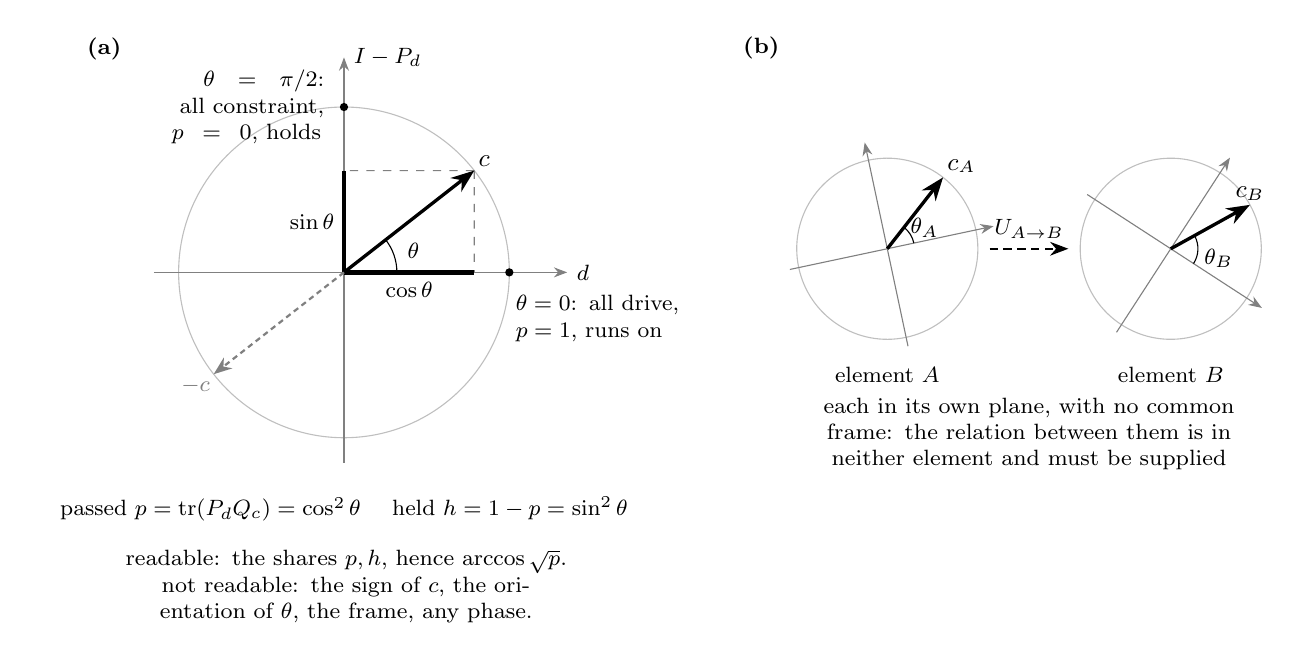
\begin{tikzpicture}[>=Stealth, font=\small]
% ---- panel (a): the comparison ----
\begin{scope}[scale=2.1]
  \draw[gray!50] (0,0) circle (1);
  \draw[->, gray] (-1.15,0) -- (1.35,0) node[right, black, font=\footnotesize] {$d$};
  \draw[->, gray] (0,-1.15) -- (0,1.3) node[right, black, font=\footnotesize] {$I-P_d$};
  \def\th{38}
  \coordinate (c) at ({cos(\th)},{sin(\th)});
  \draw[dashed, gray] (c) -- ({cos(\th)},0);
  \draw[dashed, gray] (c) -- (0,{sin(\th)});
  \draw[line width=1.6pt] (0,0) -- ({cos(\th)},0);
  \draw[line width=1.6pt] (0,0) -- (0,{sin(\th)});
  \draw[very thick, ->] (0,0) -- (c) node[above right, inner sep=1pt] {$c$};
  \draw[gray, thick, ->, dash pattern=on 2pt off 1.5pt] (0,0) -- ({-cos(\th)},{-sin(\th)}) node[below left, inner sep=1pt, font=\footnotesize] {$-c$};
  \draw (0.32,0) arc (0:\th:0.32);
  \node[font=\footnotesize] at (0.42,0.13) {$\theta$};
  \node[below, font=\footnotesize] at ({cos(\th)/2},0) {$\cos\theta$};
  \node[left, font=\footnotesize] at (0,{sin(\th)/2}) {$\sin\theta$};
  % the two ends
  \fill (1,0) circle (0.025);
  \fill (0,1) circle (0.025);
  \node[below right, font=\footnotesize, text width=2.6cm, align=left] at (0.98,-0.08) {$\theta=0$: all drive,\\ $p=1$, runs on};
  \node[left, font=\footnotesize, text width=3cm, align=right] at (-0.08,1.0) {$\theta=\pi/2$: all constraint,\\ $p=0$, holds};
  \node[below, font=\footnotesize, align=center] at (0,-1.3) {passed $p=\tr(P_dQ_c)=\cos^2\theta$ \quad held $h=1-p=\sin^2\theta$};
  \node[below, font=\footnotesize, align=center, text width=7.8cm] at (0,-1.62) {readable: the shares $p,h$, hence $\arccos\sqrt p$.\\ not readable: the sign of $c$, the orientation of $\theta$, the frame, any phase.};
  \node[font=\footnotesize\bfseries] at (-1.45,1.35) {(a)};
\end{scope}
% ---- panel (b): two elements, each in its own plane ----
\begin{scope}[xshift=6.9cm, yshift=0.3cm]
  \node[font=\footnotesize\bfseries] at (-1.6,2.55) {(b)};
  % element A
  \begin{scope}[rotate=12, scale=1.15]
    \draw[gray!50] (0,0) circle (1);
    \draw[gray, ->] (-1.1,0) -- (1.2,0);
    \draw[gray, ->] (0,-1.1) -- (0,1.2);
    \draw[very thick, ->] (0,0) -- (40:1) node[above right, inner sep=1pt] {$c_A$};
    \draw (0.3,0) arc (0:40:0.3);
    \node[font=\footnotesize] at (0.45,0.14) {$\theta_A$};
  \end{scope}
  \node[font=\footnotesize] at (0,-1.6) {element $A$};
  % element B
  \begin{scope}[xshift=3.6cm, rotate=-33, scale=1.15]
    \draw[gray!50] (0,0) circle (1);
    \draw[gray, ->] (-1.1,0) -- (1.2,0);
    \draw[gray, ->] (0,-1.1) -- (0,1.2);
    \draw[very thick, ->] (0,0) -- (62:1) node[above, inner sep=1pt] {$c_B$};
    \draw (0.3,0) arc (0:62:0.3);
    \node[font=\footnotesize] at (0.5,0.2) {$\theta_B$};
  \end{scope}
  \node[font=\footnotesize] at (3.6,-1.6) {element $B$};
  % the relation to be supplied
  \draw[thick, ->, dash pattern=on 3pt off 2pt] (1.3,0) -- (2.3,0) node[midway, above, font=\footnotesize] {$U_{A\to B}$};
  \node[font=\footnotesize, align=center, text width=5.6cm] at (1.8,-2.35) {each in its own plane, with no common frame: the relation between them is in neither element and must be supplied};
\end{scope}
\end{tikzpicture}

\caption{The element. (a) One binary comparison of the state $c$ against the measurement $d$: a unit apportioned as $\cos^2\theta$ passed and $\sin^2\theta$ held. The two ends are states of the element; what has no angle at all is a unit with one pole. What is readable is the share; the sign of $c$, the orientation of $\theta$, the frame and any phase are not. (b) Each element's angle lies in a plane of its own. The relation between two planes is in neither element. It is supplied, and in \S\ref{sec:geometry} it is a group element.}
\label{fig:element}
\end{figure}

\subsection{What is readable, and the relativity of frames}

The representation's one rule of evidence is that \textbf{only shares are readable}. The oriented angle $\theta$, the amplitudes $(\cos\theta,\sin\theta)$ with their signs, the frame in which they are written and any phase they carry are not directly readable. The unoriented acute angle $\arccos\sqrt p$ is, because the share determines it, and so is anything else the shares determine. Two states that give the same shares against every measurement are one readable state. Two consequences make the representation \emph{ordinal} rather than metric. First, $\theta$ is an angle in a plane that belongs to the element. There is no common frame in which two elements' planes could be compared directly, so the relation between two elements' frames is itself something to be supplied, across every adjacency. We call this \textbf{the relativity of frames} (Figure~\ref{fig:element}b). Second, nothing in the element carries a magnitude: a share is a share of a unit, and the unit is the element's own. If a system is to have a size, the size must be made by its composition. In a theory whose only scale is self-generated, a representation that imports none is the right starting point.

\clearpage
\section{The axioms, and what is assumed}\label{sec:axioms}

We state the representation as axioms once, in the form the results below use. Each is marked either as a \emph{postulate} of the proposed representation or as an \emph{assumption} added for the domain. A postulate is what we propose a system is, mathematically; it is not a consequence of the everyday meanings of drive and constraint, and is not claimed as one. The hypotheses are listed so that a reader can see every place where the chain from systems to gauge theory is conditional.

\begin{tcolorbox}[paperbox, title=The axioms]
\begin{description}[leftmargin=1.5em,style=nextline]
\item[A1 --- the state.] An element's state is a normalised distribution of a unit over its poles, carried as amplitudes: a unit vector in $\R^N$ (\textbf{A1$\R$}) or in $\C^N$ (\textbf{A1$\C$}), where the $N$ poles are the outcome axes of its comparisons. \emph{Postulate}, except the choice of field: \textbf{complex amplitudes are an assumption}, and \S\ref{sec:geometry} shows the real primitives do not supply them.
\item[A2 --- the readable.] What is readable of a state is the set of its shares against every measurement---the transition shares $|\langle\varphi|\psi\rangle|^2$---and nothing else; frames and phases are not readable. \emph{Postulate.}
\item[A3 --- the relation.] A relation between two frames is a bijection of the readable states that preserves every transition share; the admissible relations form a \textbf{closed, connected group} of such bijections---closed under composition and inverse, containing the identity, and connected to it by continuous paths. \emph{Postulate}, with closedness and connectedness stated rather than inferred.
\item[A3b --- transitivity.] A relation may supply any coherence: the relations act transitively on the readable states. \emph{Postulate}---it is what ``supplied in neither pole'' means---but it is an axiom, and a reader who denies it keeps a closed connected subgroup and the theorems for that subgroup.
\item[A4 --- adjacency, the interface rule, locality.] Elements are joined by interfaces; the smallest closed paths of interfaces generate all closed paths; the cost of a configuration is the sum over smallest paths of a cost depending on that path alone. \textbf{The interface rule:} the drive pole an element receives along an interface \emph{is} the previous element's held pole carried across by the relation---an element has one held pole, its own, and a drive pole per arriving interface. When the poles are live, each element of a path reads the loop from its own pole and the path's cost is the mean of the readings. \emph{Assumption}: adjacency is the content of a lattice, and MINOS does not derive space.
\item[A5 --- the dynamics.] The dynamics is Hamiltonian, kinetic plus potential, additive over interfaces and smallest paths, with one coupling. \emph{Assumption}: the form is standard and not derived; the content of each term within the form is (\S\ref{sec:central}).
\item[A6 --- composition.] A composite of elements is an element over the union of their poles, with one normalisation. A constituent's state is the restriction of the composite's amplitude vector to the constituent's poles, subnormalised; its weight is the composite's datum. A constituent of zero weight is absent. \emph{Postulate} for restriction; \textbf{the gluing of independently specified constituents into one composite is not provided and is open} (\S\ref{sec:interp}).
\item[H1 --- the loss.] The readable loss of carrying a state round a closed path is one minus the returned share, and the loss of a path is that quantity averaged over the state with the invariant measure. \emph{Hypothesis}. Another monotone function of the share gives another class function, which this paper does not show to be equivalent. The average defines an averaged model (\S\ref{sec:central}), not a sector of a fuller one (\S\ref{sec:consequence}).
\end{description}
\end{tcolorbox}

Seven axioms and one hypothesis. A1--A3b and A6 are the representation's own postulates: normalised amplitudes, transition shares as the readable, share-preserving bijections as relations, transitivity, composition by restriction. They are substantial mathematical commitments, and the representation \emph{proposes} them. A4 and A5 are the content of \emph{lattice field theory}. H1 is the choice of what to read. The precise form of the paper's claim is that the gauge structure lives entirely in the representation's postulates, and that lattice gauge theory is a severe test of what those postulates can do.

\clearpage
\section{Composing relations: the gauge geometry}\label{sec:geometry}

The relation between two elements' frames must be supplied. That the admissible relations form a closed connected group is postulated, by A3; what the axioms then determine is which group it can be, and what freedom it carries. Composed along a lattice, the relations give the gauge geometry: the local freedom, the transformation law of the links, and Gauss's law.

\subsection{The admissible relation group: its classification and local gauge freedom}

A word on notation. $G$ names the connected linear group that acts on the amplitudes: $\SU(N)$, $\SO(N)$, or one of their transitive subgroups. Its faithful action on the readable states is the quotient by the scalars it contains, $\PU(N)$ or $\PSO(N)$ and so on. The theorem states containments for the quotient and classifications for the linear group, and the text uses $G$ for both where the context makes clear which is meant.

\begin{theorem}\label{thm:group}
Under A1--A3b (A3 including closedness), A6 and the interface rule of A4:
\begin{enumerate}[label=(\roman*),leftmargin=2em]
\item (containment) the relations between frames of an $N$-pole element are induced by unitary maps of the amplitudes on the complex branch and by orthogonal maps on the real branch, and act on the readable states as a closed connected subgroup $G\subseteq\PU(N)=\SU(N)/\mathbb{Z}_N$ (complex) or $G\subseteq\SO(N)/(\SO(N)\cap\{I,-I\})\subseteq\mathrm{PO}(N)$ (real);
\item (the local freedom) every element's frame may be changed independently, so relations carry a local gauge freedom;
\item (the minimal real composite) a single two-pole element with real amplitudes has the full rotation group $\SO(2)$ of its circle; two such elements at an interface, composed under A6, have readable states forming the real projective plane $\RP^2$ with transition share $(n\cdot m)^2$, and relations generating $\SO(3)$ in its \textbf{vector} representation; the only other possibility for two real elements is one plane, $\SO(2)$. The qubit---complex amplitudes on $\CP^1$ with transition share $(1+n\cdot m)/2$---is \emph{not} obtained from two real elements;
\item (the complex branch) for an $N$-pole element with complex amplitudes, $G$ acts transitively on $\CP^{N-1}$ and is therefore $\PU(N)$ or, for even $N$, $\PSp(N/2)$, by Onishchik's classification \cite{onishchik};
\item (the real branch) for $N$ real poles, $G$ is a closed connected subgroup of $\SO(N)$ transitive on the sphere---$\SO(N)$ itself or one of the proper transitive subgroups of the Montgomery--Samelson--Borel list \cite{ms,borel}; for $N=3$ only $\SO(3)$; the group acting faithfully on $\RP^{N-1}$ is $G/(G\cap\{I,-I\})$---$\PSO(N)$ for even $N$ when $G=\SO(N)$.
\end{enumerate}
\end{theorem}

\begin{proof}[Proof (sketch; Appendix~\ref{app:proofs})]
(i) is Wigner's theorem \cite{wigner,bargmann} with antiunitaries excluded by continuity and phases quotiented by A2; (ii) is A2 applied to one element's frame; (iii) is a direct computation on the sphere of the composite's amplitudes under A6, with generation checked (check 10); (iv) and (v) are the classifications cited, applied because A3b makes the action transitive.
\end{proof}

On the real branch the non-Abelian structure is a property of a composite: one real element is $\SO(2)$, two are $\SO(3)$. On the complex branch a single two-pole element already has $\PU(2)$. And the complex amplitudes that give the qubit are nowhere derived. The representation therefore \textbf{forks}: real MINOS, with orthogonal groups on real projective spaces, and complex MINOS, with the groups of (iv). Nothing in A1--A6 selects between them. The fork is the source of the first result (\S\ref{sec:central}).

\subsection{The lattice construction, with the poles}\label{sec:construction}

Let the elements be the vertices $V$ of a graph and the interfaces its directed edges $E$. Each element $x$ carries, in its own frame, one \textbf{held pole} $c_x$---a unit amplitude vector read up to sign, a point of $\RP^{N-1}$ (real) or $\CP^{N-1}$ (complex)---which it hands across every departing interface. The relation on an edge $\ell=(x\to y)$ is an element $U_\ell\in G$, the map from $x$'s frame to $y$'s. The interface rule of A4 is the statement that the drive pole $y$ receives along $\ell$ is $x$'s held pole carried across:
\begin{equation}
d_{y,\ell}:=U_\ell c_x .
\end{equation}
The configuration space is therefore $G^E\times(\RP^{N-1})^V$ on the real branch and $G^E\times(\CP^{N-1})^V$ on the complex: the links together with the held poles. The drive poles are defined, not further variables, and this holds on every graph. A frame change $(g_x)_{x\in V}$ acts on amplitudes at $x$ by $g_x$, hence on poles by $c_x\mapsto g_xc_x$ and on relations by
\begin{equation}
U_{x\to y}\mapsto g_y\,U_{x\to y}\,g_x^{-1},
\end{equation}
the standard link transformation law, \emph{derived} from $U$ being the frame relation. The interface rule is preserved under it, so the rule is a transported label and constrains no link. The readables of an element are its \textbf{pass shares} $|\langle d_{y,\ell},c_y\rangle|^2$, one per arrival, and its \textbf{junction angles} $|\langle d_{y,\ell},d_{y,\ell'}\rangle|^2$, one per pair of arrivals. The pass share is the elemental angle of \S\ref{sec:comparison}, now seen to be a gauge invariant of the pair of elements. A vertex of higher degree adds readables, not constraints. Figure~\ref{fig:construction} shows the construction on a small graph. The Hilbert space is $L^2\big(G^E\times(\RP^{N-1})^V\big)$ ($\CP^{N-1}$ on the complex branch), and the physical space is its $G^V$-invariant subspace. The generator at $x$ is the sum of the electric fields on the edges at $x$ plus the generator of rotations of $x$'s pole, and physical states are annihilated by it. This is \textbf{Gauss's law, with the pole's charge as its source}.

\begin{figure}[!htbp]
\centering
% Figure 2: the lattice construction with the poles; the interface rule; the readables
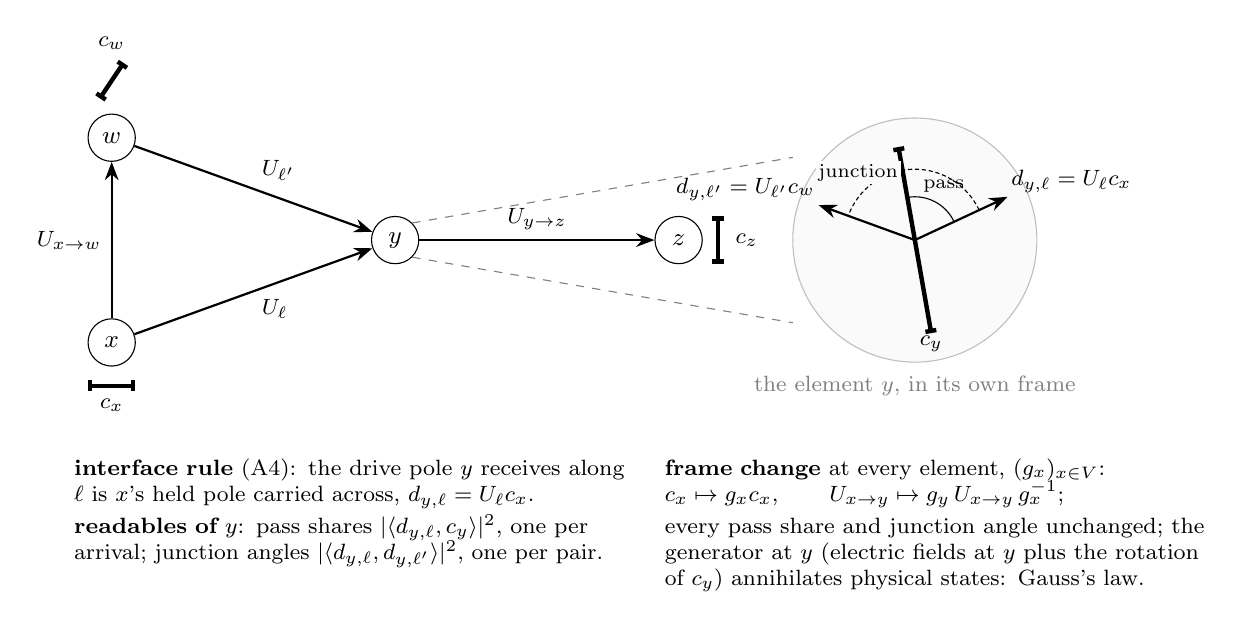
\begin{tikzpicture}[>=Stealth, font=\small,
  elem/.style={circle, draw, fill=white, minimum size=6mm, inner sep=0pt, font=\small},
  pole/.style={line width=1.6pt, {Bar[width=4pt]}-{Bar[width=4pt]}},
  drive/.style={thick, ->}]
% ---- the graph ----
\node[elem] (x) at (0,0) {$x$};
\node[elem] (w) at (0,2.6) {$w$};
\node[elem] (y) at (3.6,1.3) {$y$};
\node[elem] (z) at (7.2,1.3) {$z$};
\draw[->, thick] (x) -- node[below right=-1pt, font=\footnotesize] {$U_\ell$} (y);
\draw[->, thick] (w) -- node[above right=-1pt, font=\footnotesize] {$U_{\ell'}$} (y);
\draw[->, thick] (x) -- node[left, font=\footnotesize] {$U_{x\to w}$} (w);
\draw[->, thick] (y) -- node[above, font=\footnotesize] {$U_{y\to z}$} (z);
% held poles at x, w, z: directors (read up to sign)
\draw[pole] ($(x)+(-0.3,-0.55)$) -- ($(x)+(0.3,-0.55)$);
\node[font=\footnotesize, below] at ($(x)+(0,-0.6)$) {$c_x$};
\draw[pole] ($(w)+(-0.15,0.5)$) -- ($(w)+(0.15,0.95)$);
\node[font=\footnotesize, above] at ($(w)+(0,1)$) {$c_w$};
\draw[pole] ($(z)+(0.5,-0.3)$) -- ($(z)+(0.5,0.3)$);
\node[font=\footnotesize, right] at ($(z)+(0.6,0)$) {$c_z$};
% ---- the magnified element y ----
\coordinate (Y) at (10.2,1.3);
\draw[gray, dashed] (y.north east) -- ($(Y)+(-1.55,1.05)$);
\draw[gray, dashed] (y.south east) -- ($(Y)+(-1.55,-1.05)$);
\draw[gray!50, fill=gray!4] (Y) circle (1.55);
\node[font=\footnotesize, gray] at ($(Y)+(0,-1.85)$) {the element $y$, in its own frame};
% its held pole (director) and the two arrivals
\draw[pole] ($(Y)+(100:1.2)$) -- ($(Y)+(280:1.2)$);
\node[font=\footnotesize, below, inner sep=1pt] at ($(Y)+(280:1.2)$) {$c_y$};
\draw[drive] (Y) -- ($(Y)+(25:1.3)$) node[above right, inner sep=1pt, font=\footnotesize] {$d_{y,\ell}=U_\ell c_x$};
\draw[drive] (Y) -- ($(Y)+(160:1.3)$) node[above left, inner sep=1pt, font=\footnotesize] {$d_{y,\ell'}=U_{\ell'}c_w$};
% pass share angle between d_{y,l} and c_y ; junction angle between the two arrivals
\draw ($(Y)+(25:0.55)$) arc (25:100:0.55);
\node[font=\scriptsize] at ($(Y)+(62:0.78)$) {pass};
\draw[dash pattern=on 1.5pt off 1pt] ($(Y)+(25:0.9)$) arc (25:160:0.9);
\node[font=\scriptsize, fill=gray!4, inner sep=1pt] at ($(Y)+(130:1.12)$) {junction};
% ---- the rules, below ----
\node[align=left, font=\footnotesize, anchor=north west, text width=7cm] at (-0.6,-1.35) {%
\textbf{interface rule} (A4): the drive pole $y$ receives along $\ell$ is $x$'s held pole carried across, $d_{y,\ell}=U_\ell c_x$.\\[2pt]
\textbf{readables of $y$}: pass shares $|\langle d_{y,\ell},c_y\rangle|^2$, one per arrival; junction angles $|\langle d_{y,\ell},d_{y,\ell'}\rangle|^2$, one per pair.};
\node[align=left, font=\footnotesize, anchor=north west, text width=7cm] at (6.9,-1.35) {%
\textbf{frame change} at every element, $(g_x)_{x\in V}$:\\
$c_x\mapsto g_xc_x,\qquad U_{x\to y}\mapsto g_y\,U_{x\to y}\,g_x^{-1}$;\\[2pt]
every pass share and junction angle unchanged; the generator at $y$ (electric fields at $y$ plus the rotation of $c_y$) annihilates physical states: Gauss's law.};
\end{tikzpicture}

\caption{The construction of \S\ref{sec:construction} on a small graph. Each element carries one held pole, drawn as a director because it is read up to sign; each directed interface carries a relation. Two interfaces arrive at $y$. The drive poles they deliver are the held poles of $x$ and of $w$ carried across by $U_\ell$ and $U_{\ell'}$; the interface rule defines them, and they are not further variables. The readables of $y$ are its two pass shares and its junction angle, and the frame change shown leaves all three unchanged. The directions are drawn in a plane for legibility; the poles live in $\RP^{N-1}$ or $\CP^{N-1}$.}
\label{fig:construction}
\end{figure}

This is checked in finite dimensions, because it was contested. On the triangle (real, $N=3$), poles fixed in the frames independently of the links confine each link to a one-dimensional coset and leave no local freedom at all: three degrees of freedom, not a gauge theory. Poles transported as above leave every link free, with $\SO(3)^3$ acting freely, six degrees of freedom and six independent invariants. The fixed-pole case is recovered exactly as the transported one in the standard gauge with every pass share forced to zero (check 15). On four elements with two arrivals at one of them, the construction gives twenty variables, a free $\SO(3)^4$ orbit, eight degrees of freedom and eight invariants including the junction angle, against six under the alternative of forcing the arrivals to agree (check 16).

What the poles are: a director (real) or a ray (complex), whose frame-covariant content is the projector $Q_x=cc^{\mathsf T}$ or $\psi\psi^\dagger$, transforming as $Q_x\mapsto g_xQ_xg_x^{-1}$. Its trace is invariant, and its traceless part $Q_x-I/N$ transforms in the \textbf{traceless symmetric} representation (real) or the \textbf{adjoint} (complex), so that $Q_x$ itself carries the trivial representation plus that one---the very representations the loss will select in \S\ref{sec:central}. The projector is covariant, not invariant. The gauge invariants are traces of transported products of projectors. The simplest is the pass share $\tr(Q_yU_\ell Q_xU_\ell^{-1})$; the one the action reads is the loop's loss $1-\tr(Q_x\,WQ_xW^{-1})$, the failure of the pole's projector to return round the loop (check 16). The poles are projective matter; they are not a fundamental Higgs field, whose representation does not descend to $\PU(N)$.

\subsection{Composition, by identification or by relation}

A6 says a shared pole has one amplitude. Two systems that meet in a pole therefore compose \emph{by identification} only where they prescribe the same amplitude for it. Otherwise they compose \emph{by relation}: a junction whose readable is the overlap of the two arrivals. That overlap is one when they agree and zero when they are orthogonal, two systems that pass nothing to each other and do not collapse into one; between the two lies a share. This is why the lattice element has one held pole and a drive pole per arrival, and why a contested pole is not a contradiction. What A6 does not supply is the converse: a rule that glues independently specified comparisons, connected by arbitrary relations with arbitrary loop holonomies, into one composite state. Two constituents sharing several poles can prescribe incompatible amplitudes on them, and then no global vector exists. That gluing theorem is open, and is named in \S\ref{sec:interp} as the next task.

\clearpage
\section{The central result: under the loss rule, readable geometry determines the action's representation content}\label{sec:central}

With the relations group elements on the interfaces and the poles the elements' states, H1 reads the cost of a closed path as the loss of carrying a pole round it, averaged over the pole. The average depends on the invariant measure over the pole, which differs between the real and the complex branch, so the measure is taken first.

\subsection{The real and the complex branch have different invariant measures}

Under A2, A3 and A3b the only measure on states that no frame can distinguish is the one invariant under all relations: with $G$ transitive and compact, the unique $G$-invariant probability measure. It differs between the branches. Under A1$\R$ it is the round measure on the real sphere of amplitudes. Its push-forward to the $N$ shares is the Fisher--Rao volume of the simplex, the Dirichlet distribution with every parameter $\tfrac12$; a single share is then Beta$(\tfrac12,\tfrac{N-1}{2})$, the arcsine law when $N=2$. Under A1$\C$ it is the Fubini--Study volume on $\CP^{N-1}$. Its push-forward to the shares is uniform on the simplex, the Dirichlet distribution with every parameter $1$; a single share is Beta$(1,N-1)$, uniform only when $N=2$. The two give different averages---for the return share under $\diag(i,-i)$, $1/2$ and $1/3$ respectively (check 12)---and the first drafts of this work ran them together.

\subsection{The complex branch: the adjoint action}

\begin{theorem}\label{thm:adjoint}
Under A1$\C$, A2--A4 and H1, for an $N$-pole element with relations $U\in\SU(N)$, the readable loss round a loop is
\begin{equation}
c(U)=\E_\psi\big[1-|\langle\psi|U|\psi\rangle|^2\big]=\frac{N-1}{N}\Big(1-\frac{\chi_{\adj}(U)}{N^2-1}\Big),
\end{equation}
the Wilson action in the adjoint representation of $\SU(N)$.
\end{theorem}
\begin{proof}
$\E|\langle\psi|U|\psi\rangle|^2=(N+|\tr U|^2)/(N(N+1))$ by the second moment of the Fubini--Study measure, and $N\otimes\bar N=1\oplus\adj$ gives $|\tr U|^2=1+\chi_{\adj}$.
\end{proof}
(Check 8: $N=2$ to $5$ against Monte Carlo within error; the two forms equal to $10^{-16}$.)

\begin{remark}
Theorem~\ref{thm:adjoint} is stated for the full unitary group, $G=\PU(N)$. Theorem~\ref{thm:group}(iv) also allows $G=\PSp(N/2)$ for even $N$. The same average then holds with $U$ restricted to $\Sp(N/2)$, but the restriction of $N\otimes\bar N$ to $\Sp(N/2)$ decomposes further, into the trivial, the adjoint and the traceless antisymmetric representation, so the loss is the $\SU(N)$ adjoint character restricted to $\Sp(N/2)$ and not the symplectic adjoint alone. For $\Sp(2)$ on $\C^4$, $\mathbf4\otimes\bar{\mathbf4}=\mathbf1\oplus\mathbf5\oplus\mathbf{10}$ and $c(U)=(15-\chi_{\mathbf5}(U)-\chi_{\mathbf{10}}(U))/20$. The statement that the readable geometry fixes the representation content stands on both branches; what it fixes on the symplectic branch is this restricted character.
\end{remark}

The readable sector is therefore centre-blind: the fundamental Wilson action is not a reading of the element's own shares but of a \emph{probe} that carries a frame of its own, and the string tension of such a probe is not a quantity of the readable sector.

\subsection{The real branch: the traceless symmetric action}

\begin{theorem2p}
Under A1$\R$, A2--A4, A6 and H1, for an element or composite of $N$ real poles with relations $R\in\SO(N)$ (or a transitive subgroup of Theorem~\ref{thm:group}(v)), the readable loss round a loop is
\begin{gather}
c_{\R}(R)=\E_n\big[1-(n\cdot Rn)^2\big]=\frac{2d_S}{N(N+2)}\Big(1-\frac{\chi_S(R)}{d_S}\Big),\\
d_S=\frac{N(N+1)}{2}-1,\qquad \chi_S(R)=\frac{(\tr R)^2+\tr R^2}{2}-1,\nonumber
\end{gather}
the Wilson action in the traceless symmetric representation $S$.
\end{theorem2p}
\begin{proof}
The fourth moment of the round measure gives $\E(n\cdot Rn)^2=((\tr R)^2+N+\tr R^2)/(N(N+2))$, and $\Sym^2(N)=1\oplus S$.
\end{proof}
For $N=3$ this is $\tfrac23(1-\chi_2/5)$, the \textbf{spin-two} action, and the adjoint form $\tfrac23(1-\chi_1/3)$ does not fit (check 11, four angles to the fourth decimal; check 13, $N=3$ to $6$ within Monte Carlo error). For the full $\SO(3)$ of the minimal real three-pole composite, the traceless symmetric representation is spin two, not the spin-one adjoint, and the adjoint does not appear. For a proper transitive subgroup of Theorem~\ref{thm:group}(v) the traceless symmetric representation may decompose further and can contain adjoint components: for $\SU(2)$ acting on $\R^4$ by left multiplication on the quaternions, an element rotating two planes through $\alpha$ has $\chi_S=12\cos^2\alpha-3=3\chi_{\adj}(\alpha)$, three copies of the $\SU(2)$ adjoint, and $c_\R=\tfrac34(1-\chi_{\adj}/3)$. The distinction between the branches is a distinction in what the construction reads, not a rule that the real branch can never carry adjoint content.

\paragraph{The result.} On both branches the construction is the same: the readable state is carried round the loop, what returns is read, and the result is averaged over the frame that no one can read. When the amplitudes are complex and the group is the full unitary one, the average is the adjoint character action; on the symplectic alternative it is that character restricted (the remark after Theorem~\ref{thm:adjoint}); when the amplitudes are real it is the traceless symmetric one. The distinction between a representation and what is readable of it therefore has a definite consequence. Together with the loss rule, it decides which lattice action a system representation produces. Readability alone does not fix the action for every admissible loss; under H1 it fixes the representation content, and differently on the two branches. The character decompositions and the moment formulae are known mathematics (the complex formula is the average-gate-fidelity integral), and we claim nothing for them. What is ours is the construction that selects them, and the fork it exposes. Figure~\ref{fig:fork} sets the two branches side by side.

\begin{figure}[!htbp]
\centering
% Figure 3: the loop loss, and the fork between the real and the complex branch
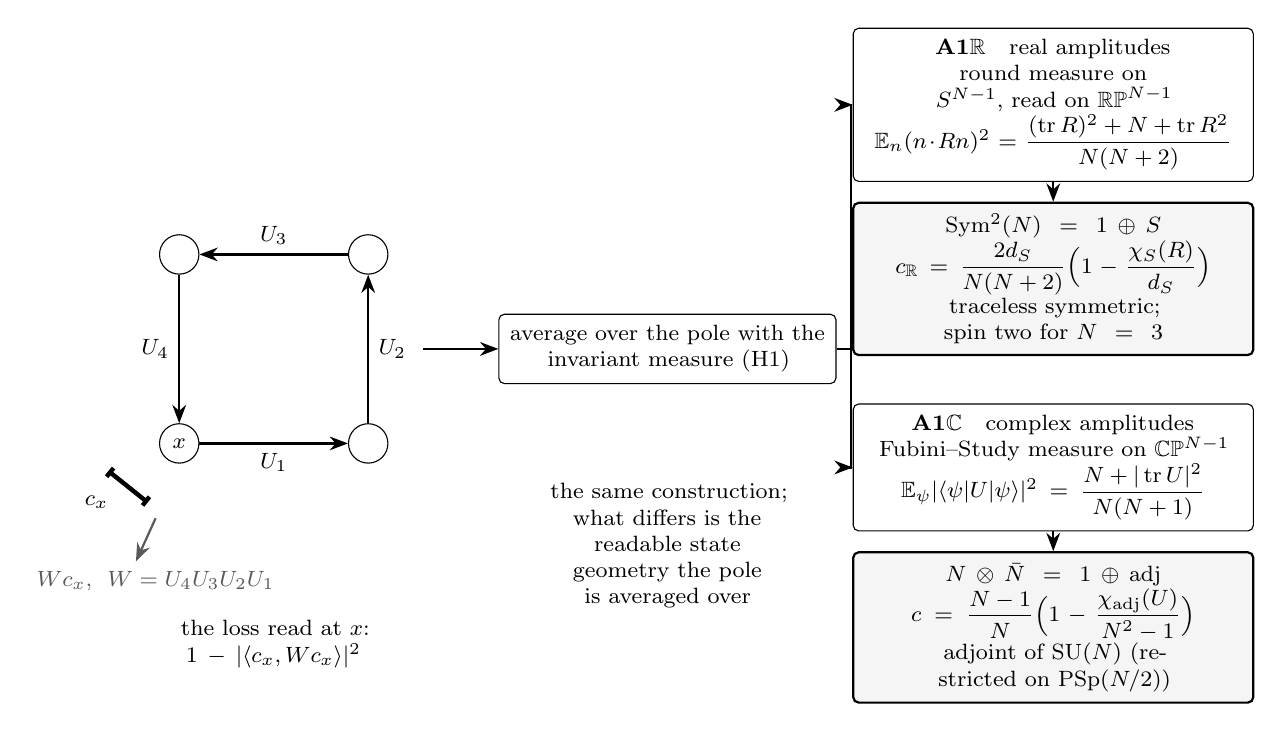
\begin{tikzpicture}[>=Stealth, font=\small,
  elem/.style={circle, draw, fill=white, minimum size=5mm, inner sep=0pt, font=\footnotesize},
  box/.style={draw, rounded corners=2pt, align=center, font=\footnotesize, inner sep=4pt},
  res/.style={box, thick, fill=gray!8}]
% ---- the plaquette ----
\begin{scope}
  \node[elem] (a) at (0,0) {$x$};
  \node[elem] (b) at (2.4,0) {};
  \node[elem] (c) at (2.4,2.4) {};
  \node[elem] (d) at (0,2.4) {};
  \draw[->, thick] (a) -- node[below, font=\footnotesize] {$U_1$} (b);
  \draw[->, thick] (b) -- node[right, font=\footnotesize] {$U_2$} (c);
  \draw[->, thick] (c) -- node[above, font=\footnotesize] {$U_3$} (d);
  \draw[->, thick] (d) -- node[left, font=\footnotesize] {$U_4$} (a);
  % the pole, carried round and returned
  \draw[line width=1.6pt, {Bar[width=4pt]}-{Bar[width=4pt]}] ($(a)+(-0.9,-0.35)$) -- ($(a)+(-0.4,-0.75)$);
  \node[font=\footnotesize] at ($(a)+(-1.05,-0.75)$) {$c_x$};
  \draw[thick, ->, gray!70!black] ($(a)+(-0.3,-0.95)$) -- ($(a)+(-0.55,-1.5)$);
  \node[font=\footnotesize, gray!70!black, anchor=north] at ($(a)+(-0.3,-1.5)$) {$Wc_x$,\ \ $W=U_4U_3U_2U_1$};
  \node[font=\footnotesize, align=center, text width=4.3cm] at (1.2,-2.55) {the loss read at $x$:\\ $1-|\langle c_x,Wc_x\rangle|^2$};
\end{scope}
% ---- the two branches ----
\node[box, text width=4.8cm] (r1) at (11.1,4.3) {\textbf{A1$\R$}\quad real amplitudes\\ round measure on $S^{N-1}$, read on $\RP^{N-1}$\\ $\E_n(n\!\cdot\!Rn)^2=\dfrac{(\tr R)^2+N+\tr R^2}{N(N+2)}$};
\node[res, text width=4.8cm, below=2.5mm of r1] (r2) {$\Sym^2(N)=1\oplus S$\\ $c_\R=\dfrac{2d_S}{N(N+2)}\Big(1-\dfrac{\chi_S(R)}{d_S}\Big)$\\ traceless symmetric; spin two for $N=3$};
\node[box, text width=4.8cm, below=6mm of r2] (c1) {\textbf{A1$\C$}\quad complex amplitudes\\ Fubini--Study measure on $\CP^{N-1}$\\ $\E_\psi|\langle\psi|U|\psi\rangle|^2=\dfrac{N+|\tr U|^2}{N(N+1)}$};
\node[res, text width=4.8cm, below=2.5mm of c1] (c2) {$N\otimes\bar N=1\oplus\adj$\\ $c=\dfrac{N-1}{N}\Big(1-\dfrac{\chi_{\adj}(U)}{N^2-1}\Big)$\\ adjoint of $\SU(N)$ (restricted on $\PSp(N/2)$)};
% ---- the average, placed between the branches ----
\node[box, text width=4cm] (avg) at (6.2,1.2) {average over the pole with the\\ invariant measure (H1)};
\draw[->, thick] (3.1,1.2) -- (avg);
\draw[->, thick] (avg.east) -- ++(0.18,0) |- (r1.west);
\draw[->, thick] (avg.east) -- ++(0.18,0) |- (c1.west);
\draw[->, thick] (r1) -- (r2);
\draw[->, thick] (c1) -- (c2);
\node[font=\footnotesize, align=center, text width=4.2cm] at (6.2,-1.3) {the same construction;\\ what differs is the readable state\\ geometry the pole is averaged over};
\end{tikzpicture}

\caption{The loss round a closed path, and the fork. The held pole at $x$ is carried round the smallest path and compared with itself on return; the readable loss is one minus the returned share. H1 averages that loss over the pole with the invariant measure. The construction is the same on both branches. The measure is not, and neither is the character the average selects: traceless symmetric for real amplitudes (Theorem 2$'$), adjoint for complex (Theorem~\ref{thm:adjoint}). The fundamental appears on neither.}
\label{fig:fork}
\end{figure}

\FloatBarrier
\subsection{The kinetic term and the averaged Hamiltonian}\label{sec:averaged}

\begin{theorem}\label{thm:casimir}
Let the information distance between two relations be the readable difference between the states they produce from the same state, averaged over that state with the invariant measure:
\[
D^2(U,U')=\E_\psi\big[1-|\langle U\psi,U'\psi\rangle|^2\big]=c(U^{-1}U'),
\]
with $c$ the loss of Theorem~\ref{thm:adjoint} or $2'$. Then $D$ is bi-invariant on $G$; its infinitesimal form, where nondegenerate, is a bi-invariant Riemannian metric on $G$; and the Laplace--Beltrami operator of that metric is the quadratic Casimir of the invariant inner product it induces, the Killing form up to scale when $G$ is simple. On the linear covering group $D$ is a pseudometric, degenerate on the scalar centre ($D(I,-I)=0$ in $\SU(2)$); on the faithful projective quotient it is a metric.
\end{theorem}
(Check 9: identical to six decimals after moving both relations by the same pair of group elements; small-displacement coefficient $1.00$ against the Killing form.)

\begin{theorem}[the averaged model]\label{thm:averaged}
Under A1--A5 and H1---the poles auxiliary, the loss of a path \emph{defined} as its average over the pole---the dynamics is
\begin{equation}
H=\frac{g^2}{2}\sum_{\text{interfaces}}\Delta_\ell+\frac{1}{g^2}\sum_{\text{smallest paths}}c(U_p),
\end{equation}
with $\Delta_\ell$ the Casimir on the interface's relation and $c$ the character loss of Theorem~\ref{thm:adjoint} or $2'$, on the states invariant under independent frame changes at every element: the Kogut--Susskind Hamiltonian \cite{ks} in the adjoint reading (traceless symmetric on the real branch), with Gauss's law the invariance condition.
\end{theorem}
\emph{This is a model defined by an averaging, and the theorem says so.} What the second result amounts to is therefore a reconstruction under explicit assumptions. Given A5's form, the content of each term is forced: the Casimir by the metric, the character action by the loss. The form itself is not derived, and neither is the claim that nature's dynamics is generated by this Laplacian rather than by a function of it. (Locality, gauge invariance and continuity in the metric do not select it: $\sum(-\Delta_\ell)^2+\sum c(U_p)$ satisfies all three.)

The two readings meet at weak coupling: the fundamental and adjoint actions have the same leading local continuum term after coupling normalisation, with couplings in the ratio $2N/(N+1)$ (check 4), which is a statement about the local term and not about the global structure of $\SU(N)$ against $\PU(N)$.

\clearpage
\section{A nontrivial consequence: the projective-pole model and its induced interaction}\label{sec:consequence}

Theorem~\ref{thm:averaged} defined the loss of a path as its average over the pole. The averaging leaves something out: the poles cannot be removed from the dynamics. They are kept here as variables, and what they induce is computed.

\subsection{The poles cannot be averaged out of the dynamics}

Averaging the loss over the pole and restricting the dynamics to pole-independent states are different operations. With $P$ the projector on states independent of the poles, $PVP=c(U)P$---the character action---but $(I-P)VP\neq0$: on one $\SO(3)$ plaquette with one pole, for the quarter turn, $PVP=0.800000=\tfrac23(1-\chi_2/5)$ while $\|(I-P)VP\|=0.2667$, the standard deviation of the loss over the pole (check 17). A pole-independent state leaves the subspace at once. \textbf{There is no pole-neutral sector of the full dynamics.} The pure theory of Theorem~\ref{thm:averaged} is the averaged model, or---as follows---the leading term of a limit.

\subsection{The reduction, and the two-plaquette kernel}

\begin{theorem4p}
Let the poles be dynamical with their own kinetic term---by Theorem~\ref{thm:casimir} on the pole's state space, the Laplacian of its invariant metric, with coefficient $\kappa$---so that the full Hamiltonian is
\begin{equation}
H_{\mathrm{full}}=\frac{g^2}{2}\sum_\ell\Delta_\ell+\kappa\sum_x\Delta_{\mathrm{pole},x}+\frac{1}{g^2}\sum_pV_p,\qquad V_p=\frac{1}{|p|}\sum_{x\in p}V\big(W_p^{(x)},n_x\big),
\end{equation}
with $V_p$ the loss of path $p$ read from each of its $|p|$ elements and averaged (A4). Then, as a formal low-energy asymptotic expansion for a fixed finite graph in a window of bounded link energy,
\begin{gather}
E_0(U;\kappa)=\frac{1}{g^2}\sum_pc(U_p)-\frac{1}{\kappa g^4}\sum_x\sum_{p,q\ni x}\frac{K\big(V_p^{(x)},V_q^{(x)}\big)}{|p|\,|q|}+O(\kappa^{-2}),\\
K(V_1,V_2)=\sum_{m\neq0}\frac{\langle0|V_1|m\rangle\langle m|V_2|0\rangle}{\lambda_m},\nonumber
\end{gather}
the inner sum over ordered pairs of smallest paths through $x$ and $\lambda_m$ the pole Laplacian's eigenvalues. The leading term is the character action. The next is a sum of one-plaquette corrections ($p=q$), which are class functions, and of \textbf{two-plaquette interactions} ($p\neq q$) wherever two paths are read through one pole. Each two-plaquette term is a function of the pair of holonomies based at the shared element; it is invariant under their simultaneous conjugation and not determined by their separate classes.
\end{theorem4p}

\paragraph{The kernel in closed form (real branch, $N=3$).} For a rotation through $\varphi$ about the axis $a$, $n\cdot Rn=t+(1-t)(n\cdot a)^2$ with $t=\cos\varphi$, so the loss has harmonics of degree $0$, $2$ and $4$ only, with zonal coefficients
\begin{equation}
A_2(t)=-\tfrac{4}{21}(1-t)(4t+3),\qquad A_4(t)=-\tfrac{8}{35}(1-t)^2,
\end{equation}
and by the addition theorem
\begin{equation}\label{eq:kernel}
K(R_1,R_2)=\frac{A_2(t_1)A_2(t_2)}{30}\,P_2(a\cdot b)+\frac{A_4(t_1)A_4(t_2)}{180}\,P_4(a\cdot b).
\end{equation}
For two quarter turns, $K=\tfrac{8}{735}P_2(a\cdot b)+\tfrac{16}{55125}P_4(a\cdot b)$: $+0.0111746$ for parallel axes, $-0.0053333$ for perpendicular; a quarter turn beside a half turn gives $-16/2625$ even for parallel axes. Under A4's average a plaquette of $L$ elements has its own second-order coefficient $K_1/L$, $0.00279365$ for a quarter-turn square. Figure~\ref{fig:kernel} plots the kernel.

\begin{figure}[!htbp]
\centering
% Figure 4: two plaquettes read through one pole, and the induced two-plaquette kernel
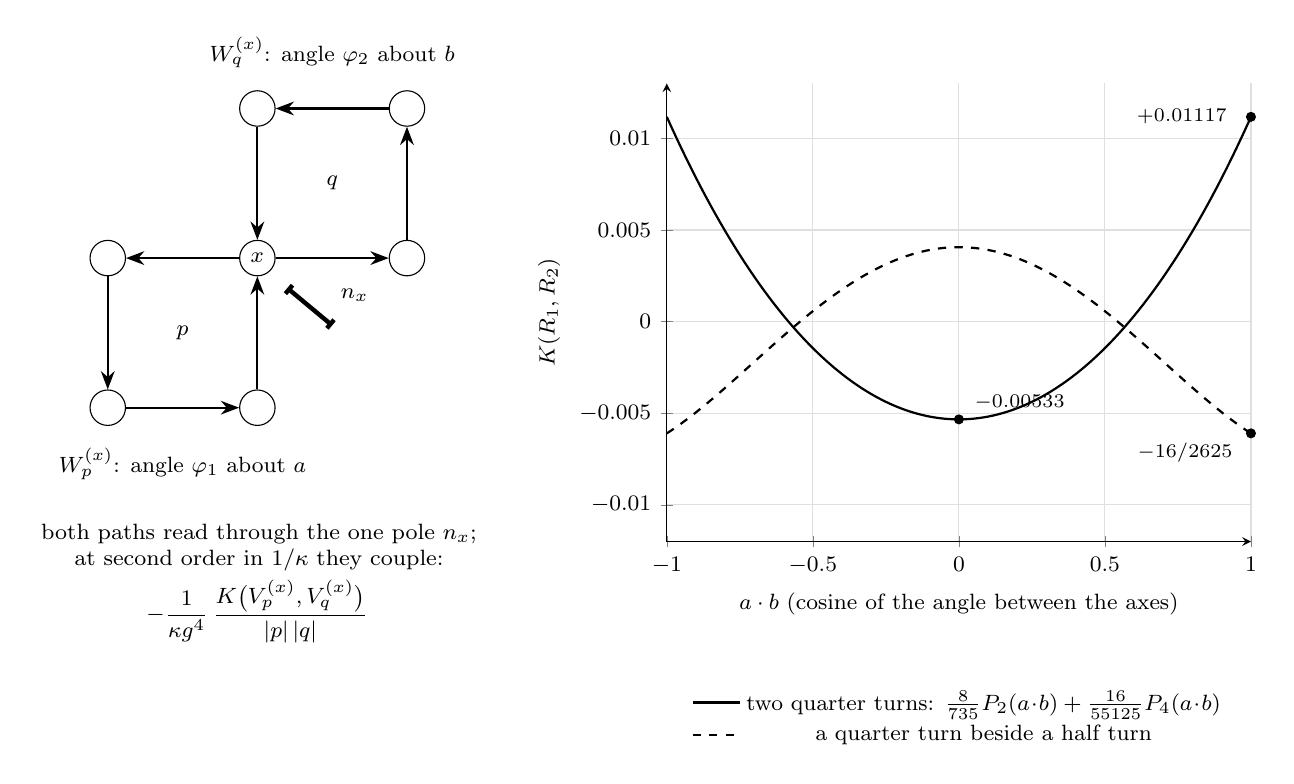
\begin{tikzpicture}[>=Stealth, font=\small,
  elem/.style={circle, draw, fill=white, minimum size=4.5mm, inner sep=0pt, font=\footnotesize}]
% ---- two squares sharing the element x ----
\begin{scope}[scale=0.95]
  \node[elem] (x) at (0,0) {$x$};
  \node[elem] (p1) at (-2,0) {};
  \node[elem] (p2) at (-2,-2) {};
  \node[elem] (p3) at (0,-2) {};
  \node[elem] (q1) at (2,0) {};
  \node[elem] (q2) at (2,2) {};
  \node[elem] (q3) at (0,2) {};
  \draw[thick, ->] (x) -- (p1); \draw[thick, ->] (p1) -- (p2); \draw[thick, ->] (p2) -- (p3); \draw[thick, ->] (p3) -- (x);
  \draw[thick, ->] (x) -- (q1); \draw[thick, ->] (q1) -- (q2); \draw[thick, ->] (q2) -- (q3); \draw[thick, ->] (q3) -- (x);
  \node[font=\footnotesize] at (-1,-1) {$p$};
  \node[font=\footnotesize] at (1,1) {$q$};
  \node[font=\footnotesize, align=left] at (-1,-2.75) {$W_p^{(x)}$: angle $\varphi_1$ about $a$};
  \node[font=\footnotesize, align=left] at (1,2.75) {$W_q^{(x)}$: angle $\varphi_2$ about $b$};
  % the pole at x
  \draw[line width=1.6pt, {Bar[width=4pt]}-{Bar[width=4pt]}] ($(x)+(0.4,-0.4)$) -- ($(x)+(1.0,-0.9)$);
  \node[font=\footnotesize] at ($(x)+(1.3,-0.5)$) {$n_x$};
  \node[font=\footnotesize, align=center, text width=5.6cm] at (0,-4.35) {both paths read through the one pole $n_x$;\\ at second order in $1/\kappa$ they couple:\\[2pt] $-\dfrac{1}{\kappa g^4}\,\dfrac{K\big(V_p^{(x)},V_q^{(x)}\big)}{|p|\,|q|}$};
\end{scope}
% ---- the kernel ----
\begin{scope}[xshift=5.2cm, yshift=-3.6cm]
\begin{axis}[
  width=9cm, height=7.4cm,
  xlabel={$a\cdot b$ (cosine of the angle between the axes)},
  ylabel={$K(R_1,R_2)$},
  xmin=-1, xmax=1, ymin=-0.012, ymax=0.013,
  xtick={-1,-0.5,0,0.5,1},
  ytick={-0.01,-0.005,0,0.005,0.01},
  yticklabel style={/pgf/number format/fixed, /pgf/number format/precision=3},
  scaled y ticks=false,
  grid=major, grid style={gray!25},
  axis lines=left,
  legend style={at={(0.5,-0.3)}, anchor=north, draw=none, font=\footnotesize, legend columns=1},
  tick label style={font=\footnotesize}, label style={font=\footnotesize},
  samples=121, domain=-1:1, no markers]
  % quarter turn beside quarter turn: (8/735) P2 + (16/55125) P4
  \addplot[thick, black] {8/735*(3*x^2-1)/2 + 16/55125*(35*x^4-30*x^2+3)/8};
  % quarter turn beside half turn: A2(0)A2(-1)/30 P2 + A4(0)A4(-1)/180 P4
  \addplot[thick, black, dashed] {-32/4410*(3*x^2-1)/2 + 256/220500*(35*x^4-30*x^2+3)/8};
  \addplot[only marks, mark=*, mark size=1.6pt, black] coordinates {(1,0.0111746) (0,-0.0053333) (1,-0.0060952)};
  \node[font=\scriptsize, anchor=east] at (axis cs:0.95,0.0111746) {$+0.01117$};
  \node[font=\scriptsize, anchor=south west] at (axis cs:0.02,-0.0053333) {$-0.00533$};
  \node[font=\scriptsize, anchor=north east] at (axis cs:0.97,-0.0060952) {$-16/2625$};
  \legend{two quarter turns: $\tfrac{8}{735}P_2(a\!\cdot\!b)+\tfrac{16}{55125}P_4(a\!\cdot\!b)$, a quarter turn beside a half turn}
\end{axis}
\end{scope}
\end{tikzpicture}

\caption{Two smallest paths through one element, and the interaction they induce. Left: the paths $p$ and $q$ are both read through the pole $n_x$, and at second order in $1/\kappa$ the pole couples them (Theorem 4$'$). Right: the kernel of equation~(\ref{eq:kernel}) for two quarter turns, against the cosine of the angle between their axes, and for a quarter turn beside a half turn. The marked values are those quoted in the text and in check 18. $K$ enters the ground energy with the negative prefactor of Theorem 4$'$, as $-K/(\kappa g^4|p|\,|q|)$, so a positive $K$ lowers the energy. No coefficient in either curve is free.}
\label{fig:kernel}
\end{figure}

\paragraph{What is fixed.} The two-plaquette interaction has no coefficient of its own. Its size relative to the one-plaquette correction, its sign, and its dependence on the two angles and the relative axis are all fixed by the pole being projective matter in the vector representation with H1's quartic loss. The free numbers of the model are $g$ and $\kappa$. The stiffness $\kappa$ is a second number the axioms do not fix. This is the third result: once the model is specified, these quantities are determined. Integrating out stiff matter to induce gauge interactions is an established subject \cite{km,ps}; we have neither found nor excluded an exact prior match for this kernel, and we claim only that the construction fixes it.

\paragraph{What the model is, and is not.} $H_{\mathrm{full}}$ gives the poles a kinetic term and the loop losses, and nothing else. With every holonomy trivial the potential vanishes whatever the poles' arrangement, so the projective field has no spatial stiffness of its own. A hopping term $\tr(Q_yU_\ell Q_xU_\ell^{-1})$, the gauged $\CP^{N-1}$ model's \cite{cpn}, is gauge-invariant and available. A4 and A5 put the potential on closed paths only, which is why it is absent; nothing in the axioms derives such a term and nothing forbids it. The stated theory is a specialised member of the family ``gauge theory coupled to projective matter''. Making the poles stiff is not a continuum limit: $\kappa\to\infty$ gives the pure lattice theory on the graph, and nothing here concerns four dimensions or $a\to0$.

\clearpage
\section{Verification}\label{sec:verification}

The computations behind the results, the checks that carry the argument, and the two faults found and corrected are recorded here.

\subsection{One script produces every number in the paper}

All reported numerical checks are generated by the one accompanying script, seeded, in about fifteen minutes with numpy and scipy, and written to \texttt{results.txt} and \texttt{results.json} beside it. Table~\ref{tab:checks} lists the checks that carry the argument.

\begin{table}[!htbp]
\centering\small
\caption{The checks that carry the argument, what each establishes, and its result.}
\label{tab:checks}
\begin{tabular}{@{}>{\raggedright\arraybackslash}p{1.4cm}>{\raggedright\arraybackslash}p{7.6cm}>{\raggedright\arraybackslash}p{6.2cm}@{}}
\toprule
check & what it establishes & result\\
\midrule
8 & Theorem~\ref{thm:adjoint}'s second moment and the adjoint form, $N=2$--$5$ & Monte Carlo within error; forms equal to $10^{-16}$\\
11, 13 & Theorem $2'$: the spin-two action for $N=3$; the traceless symmetric action for $N=3$--$6$ & to the fourth decimal; within error\\
12 & the two invariant measures told apart on $\diag(i,-i)$ & $1/3$ and $1/2$\\
9 & Theorem~\ref{thm:casimir}: bi-invariance and the Casimir coefficient & six decimals; $1.00$\\
15 & the interface rule against the free link on the triangle & fixed poles 3 d.o.f.; transported 6; coset $=$ zero-pass-share sector\\
16 & the general graph with two arrivals at one element & 8 d.o.f., 8 invariants; the constrained alternative 6\\
17 & no pole-neutral sector; the one-pole stiffness expansion & $PVP=0.8$; $\|(I-P)VP\|=0.2667$; $\kappa(c-E_0)\to0.01118$ against $0.01117$\\
18, 19(a) & the two-plaquette kernel, quarter turns at five angles and arbitrary angles & to $10^{-16}$; $-16/2625$ recovered\\
19(b) & the complete A4-averaged fixed-link Hamiltonian on two squares sharing an element, every pole kept & $K_1/4.00$; residual$\times\kappa^2=-0.00004$ at every $\kappa$ from 10 to 160\\
20, 21 & the reduction with the link dynamical: one plaquette's link-and-pole Hamiltonian diagonalised directly against the effective operator, across truncations to 18\,876 states, in the gauge-invariant sector, four lowest levels & residual$\times\kappa^2$ steady at $0.0022$--$0.0028$ across $\kappa=5$--$80$\\
\bottomrule
\end{tabular}
\end{table}

\subsection{The two strongest checks, and the two faults found and corrected}

The strongest of these are 19(b) and 21: the first tests the whole finite-graph Hamiltonian rather than its components, the second lets the link move quantum mechanically and compares spectra rather than one energy. Both are numerical evidence on fixed graphs, not operator theorems, and are described so. Two instrument faults found during the checks are kept in the results with their corrected forms. One was an effective operator first compared against the exact kernel function rather than one formed in the same truncation; it produced a $1/\kappa$ residual at small $g$ that was the truncation's. The other was a generator convention that failed to commute with the potential; it was found by testing the commutator and replaced by the one that commutes to $10^{-13}$. Appendix~\ref{app:loop} gives the adjunct results on the smallest closed loop with the same standard.

\clearpage
\section{Interpretation and limits}\label{sec:interp}

The results are sorted here by kind, with what has been shown, what has not, and what is left open.

\subsection{Which results are known mathematics, which are the representation's, and which are demonstrated}

Table~\ref{tab:kinds} separates what is established mathematics, what the representation contributes, and what the paper demonstrates.

\begin{table}[!htbp]
\centering\small
\caption{Three kinds of result.}
\label{tab:kinds}
\begin{tabular}{@{}>{\raggedright\arraybackslash}p{3.6cm}>{\raggedright\arraybackslash}p{11.6cm}@{}}
\toprule
category & what it is here\\
\midrule
\textbf{established mathematics} & Wigner's theorem and the transitive-group classifications; character decomposition and invariant integration; the Casimir as the bi-invariant Laplacian; degenerate perturbation theory and the Schur complement\\
\addlinespace
\textbf{the representation's contribution} & an operational organisation of these tools around a primitive comparison, a rule of what is readable, and relations supplied between frames---under which the group, the local freedom, Gauss's law, the measure, the actions and the kinetic term are produced in sequence, with the real/complex fork exposed\\
\addlinespace
\textbf{demonstrated usefulness} & the construction yields coherent gauge-invariant models on any graph; what is readable selects representation-dependent actions; with the poles live, it fixes a particular induced interaction whose form is not a free choice; and every step was made precise enough to be checked, and was\\
\bottomrule
\end{tabular}
\end{table}

\subsection{What is derived, reconstructed, and model-dependent}

\emph{Derived} from the representation's postulates: given A3's group, the permitted gauge groups and their faithful action on the readable states (Theorem~\ref{thm:group}); the local gauge freedom and the transformation law of the links; Gauss's law with the pole charge; the invariant measure; the character actions under H1 (Theorems~\ref{thm:adjoint}, $2'$); the Casimir as the natural Laplacian (Theorem~\ref{thm:casimir}). \emph{Reconstructed} under assumptions: the Hamiltonian (Theorem~\ref{thm:averaged} needs A5's form and H1's average). \emph{Consequences of the specified model}: Theorem $4'$ and its kernel. \emph{Hypotheses throughout}: complex amplitudes; transitivity; adjacency; the kinetic-plus-potential form; the loss functional; the poles' stiffness.

\subsection{What remains open, and is not claimed}

\begin{itemize}[leftmargin=1.5em]
\item \textbf{The composition law.} A6 restricts a given composite; it does not glue independently specified comparisons with arbitrary holonomies into one. Defining that operation, and finding which constraints it imposes, is the next mathematical task; it is also the point at which the representation's own content, rather than its organisation of known content, would be tested.
\item \textbf{Complex amplitudes} remain a hypothesis; the minimal real composite gives $\SO(3)$ in its vector representation on $\RP^2$ and a spin-two action, not the qubit.
\item \textbf{Whether the fixed interaction is a restriction} competing gauge--matter models lack, or a rediscovery within them, awaits a literature comparison we have not made.
\item \textbf{The continuum theory and the mass gap} are untouched. Nothing here bears on four dimensions, on $a\to0$, or on the spectrum of the continuum theory, and we make no claim about them.
\end{itemize}

\subsection{Conclusion}

The paper set out to test a representation of systems in a domain that does not forgive a loose statement, and it reports a first test that the representation passes, with the qualifications given. With its postulates and its domain assumptions separated and listed, the representation produces the gauge-covariant relations, the readable observables and the lattice actions in sequence, and each step either follows from the postulates or rests on a named assumption. In the projective-pole model it goes one step further and fixes an interaction whose form can be computed, and was.

The results do not give Yang--Mills theory a new foundation, and they predict nothing. What they show is narrower. A representation devised for systems in general can be stated precisely, carried into an established mathematical theory, and used there to construct and analyse structure without renaming the theory's objects. In the other direction, the theory's structures can be understood as consequences of a few statements about systems together with the postulates and assumptions listed in \S\ref{sec:axioms}, which is the explanatory purpose the paper set itself.

Whether the representation is a good account of systems in general remains open. So does the question that would test its own content rather than its organisation of known content: whether its rule of composition restricts gauge theory beyond what the theory already allows. This paper is the first case in which the representation is stated plainly enough for that question to be put.

\appendix

\clearpage
\section{Proofs}\label{app:proofs}

\paragraph{Theorem~\ref{thm:group}.}
\begin{enumerate}[label=(\roman*), leftmargin=2em, itemsep=4pt]
\item \emph{Containment.} By A2 the readable is the set of transition shares, and by A3 a relation preserves all of them. Wigner's theorem states that a bijection of projective space preserving all transition shares is induced by a unitary or an antiunitary map, unique up to phase. Antiunitaries are not connected to the identity, and A3's continuity excludes them. A phase induces the same map on readable states, so relations act through $\PU(N)$. The admissible set is closed by A3, and connected because it is reached by continuous composition from the identity.
\item \emph{The local freedom.} A change of frame at $x$, applied to every relation touching $x$, changes nothing readable. So $U_\ell\mapsto g_yU_\ell g_x^{-1}$, with the $g$ independent from element to element, is a symmetry.
\item \emph{The minimal real composite.} A real two-pole element has states on the unit circle read up to sign, $\RP^1$; its readable-preserving connected maps form $\SO(2)$, transitive by A3b.

Two such elements, $A$ with poles $(x,y)$ and $B$ with poles $(y,z)$, meet at an interface and compose under A6 into one element over $(x,y,z)$ with one normalisation. Its amplitudes are a unit vector $n\in S^2$, read up to sign: $\RP^2$. $A$'s state is the restriction $(n_x,n_y)$, with weight $n_x^2+n_y^2$; $B$'s is $(n_y,n_z)$. The unnormalised restrictions exist everywhere; the normalised constituent states are undefined exactly at the measure-zero points where the weight vanishes, and there the constituent is absent.

$A$'s relations rotate the $(x,y)$ plane and $B$'s the $(y,z)$ plane. Rotations about two distinct axes generate $\SO(3)$ (check 10). The transition share between the readable states $\pm n$ and $\pm m$ is $(n\cdot m)^2$, the vector representation.

$\RP^2$ and $\CP^1$ are not homeomorphic, and their transition shares differ, so the qubit is not obtained.
\item \emph{The complex branch.} $G\subseteq\PU(N)$ acts transitively on $\CP^{N-1}$ by A3b. The compact connected groups transitive on $\CP^{N-1}$ are $\SU(N)$ and, for even $N$, $\Sp(N/2)$, up to the kernel \cite{onishchik}.
\item \emph{The real branch.} The connected readable-preserving maps are $\SO(N)$. A3b makes the action transitive on $\RP^{N-1}$, hence on $S^{N-1}$. The transitive compact connected groups on spheres are classified \cite{ms,borel}. $-I$ acts trivially on $\RP^{N-1}$.\qed
\end{enumerate}

\paragraph{Theorem~\ref{thm:adjoint}.}
\begin{itemize}[leftmargin=2em, itemsep=3pt]
\item For $\psi$ distributed by the Fubini--Study measure, the second moment is $\E[\psi_i\bar\psi_j\psi_k\bar\psi_l]=(\delta_{ij}\delta_{kl}+\delta_{il}\delta_{kj})/(N(N+1))$.
\item Contracting with $U_{ji}\bar U_{lk}$ gives $\E|\langle\psi|U|\psi\rangle|^2=(N+|\tr U|^2)/(N(N+1))$.
\item $N\otimes\bar N=1\oplus\adj$ gives $|\tr U|^2=1+\chi_{\adj}(U)$, and the formula follows.\qed
\end{itemize}

\paragraph{Theorem $2'$.}
\begin{itemize}[leftmargin=2em, itemsep=3pt]
\item On $S^{N-1}$ the fourth moment is $\E[n_in_jn_kn_l]=(\delta_{ij}\delta_{kl}+\delta_{ik}\delta_{jl}+\delta_{il}\delta_{jk})/(N(N+2))$, so $\E(n\cdot Rn)^2=((\tr R)^2+N+\tr R^2)/(N(N+2))$.
\item $\Sym^2(N)=1\oplus S$, with character $((\tr R)^2+\tr R^2)/2=1+\chi_S$. Hence $1-\E(n\cdot Rn)^2=(2/(N(N+2)))(d_S-\chi_S)$.
\item For a proper transitive subgroup the round measure is still the invariant one, and the formula holds with $\chi_S$ restricted.\qed
\end{itemize}

\paragraph{Theorem~\ref{thm:casimir}.}
\begin{itemize}[leftmargin=2em, itemsep=3pt]
\item By unitarity (orthogonality on the real branch), $|\langle U\psi,U'\psi\rangle|^2=|\langle\psi,U^{-1}U'\psi\rangle|^2$, so $D^2(U,U')=c(U^{-1}U')$, with $c$ the averaged return loss. $c$ is a class function, by the invariance of the measure.
\item Left translation, $U\mapsto gU$ and $U'\mapsto gU'$, leaves $U^{-1}U'$ unchanged. Right translation conjugates it, and $c$ is a class function. So $D$ is bi-invariant.
\item The second-order expansion of $D^2$ about $U'=U$ is a bi-invariant quadratic form on the Lie algebra, nondegenerate wherever $c$ is nondegenerate at the identity; check 9 finds its coefficient $1.00$ against the Killing form for $\SU(2)$. It is therefore a bi-invariant Riemannian metric.
\item The Laplace--Beltrami operator of a bi-invariant metric on a compact Lie group is the quadratic Casimir of the corresponding invariant inner product \cite{helgason}. For a compact simple group that inner product is the Killing form up to scale. For a transitive group of Theorem~\ref{thm:group} that is not simple, the Casimir is the one of the inner product that $D$ induces.\qed
\end{itemize}

\paragraph{Theorem~\ref{thm:averaged}.}
\begin{itemize}[leftmargin=2em, itemsep=3pt]
\item \emph{Kinetic term.} Theorem~\ref{thm:casimir}, with A5's form.
\item \emph{Potential.} Theorem~\ref{thm:adjoint} or $2'$ with A4: under H1's average it is a function of the links alone.
\item \emph{Invariance.} By A2, two states of the relations that differ by a frame change at an element are one readable state. The generators, the electric fields summed at an element, therefore annihilate physical states.\qed
\end{itemize}

\paragraph{Theorem $4'$.}
\begin{itemize}[leftmargin=2em, itemsep=3pt]
\item \emph{Fixed links.} At fixed links the poles decouple, and each pole's Hamiltonian is $\kappa\Delta+g^{-2}\sum_{p\ni x}V_p^{(x)}/|p|$. Degenerate perturbation theory about the uniform ground state, whose gap is $\kappa\lambda_1$, gives at second order
\[
-\frac{1}{\kappa g^4}\sum_{m\neq0}\frac{\big|\langle m|\sum_pV_p^{(x)}/|p|\,|0\rangle\big|^2}{\lambda_m}.
\]
Expanding the square gives the double sum. Poles at different elements are independent, so only paths through a common element couple. Invariance under simultaneous conjugation follows from the invariance of the measure and of the Laplacian.
\item \emph{Links dynamical.} The same expansion is the Schur complement of the pole-excited block. Its resolvent is $1/(\kappa\lambda_m)$ plus terms carrying the link Laplacian, of relative order $g^2/(\kappa\lambda_m)$, which enter at $O(\kappa^{-2})$ within a window of bounded link energy. Checks 20 and 21 test this, and the operator statement is not claimed beyond that window.
\item \emph{The closed-form kernel.} $V_{\varphi,a}(n)=1-[t+(1-t)(n\cdot a)^2]^2$, expanded in Legendre polynomials of $n\cdot a$, gives the zonal coefficients $A_2$ and $A_4$. The addition theorem $\sum_mY_{\ell m}(a)\bar Y_{\ell m}(b)=(2\ell+1)P_\ell(a\cdot b)/4\pi$ and $\lambda_\ell=\ell(\ell+1)$ then give $K$.\qed
\end{itemize}

\clearpage
\section{The smallest closed loop (adjunct results)}\label{app:loop}

For $\SU(2)$ and one loop, $H=\lambda C_2+v(U)/\lambda$ on class functions, with $v$ the amplitude (fundamental) or the share (adjoint) cost matched at weak coupling (check 6). In the share reading the potential never populates half-integer $j$: the vacuum sector of the readable reading contains only whole carriers, an exact selection rule at every coupling. At strong coupling the ratio of the two readings' gaps tends to $C_2(1)/C_2(\tfrac12)=8/3=C_A/C_F$---the first excitation of a loop is the fundamental carrier under the amplitude reading and the adjoint carrier under the share reading, at strong coupling---and at weak coupling the ratio tends to one, as the common leading local term requires. The lattice values of the lightest glueball mass in units of the square root of the string tension across $\SU(N)$ \cite{lt,teper} vary with $N$ in the direction, and roughly by the amount, that $\sqrt{C_A/C_F}$ would give; in this representation that would read as the carrier of the lowest excitation being the adjoint one. We record the comparison as a reading: the proportionality constant is not derived, and the scaling is not claimed as a result here.

Prepared as the ground state at coupling $2\lambda$ and evolved at coupling $\lambda$, the loop is neutral at every instant---neutrality is preserved by the gauge-invariant evolution---and the expectation of its held share oscillates about a non-zero mean. Its dominant frequency is the gap of $H$ to four decimals at $\lambda=0.5,1,2$; the exact spectral content (check 7) is that the prepared state's weight in the ground and first connected excited state is $0.99998$, $1.000000$, $1.000000$ and the gap frequency carries the same share of the alternating power, the remainder sitting at the other transition frequencies. The two-level description holds to those figures and no better, and an exact single-frequency statement would need a selection rule we do not have.

\begingroup\small\setlength{\parskip}{0pt}
\begin{thebibliography}{12}\setlength{\itemsep}{1pt}
\bibitem{krs} G.~S. Kirk, J.~E. Raven and M.~Schofield, \emph{The Presocratic Philosophers}, 2nd ed., Cambridge University Press (1983), ch.~VI; the fragments are numbered as in Diels--Kranz.
\bibitem{wigner} E.~P. Wigner, \emph{Gruppentheorie und ihre Anwendung auf die Quantenmechanik der Atomspektren}, Vieweg (1931).
\bibitem{bargmann} V.~Bargmann, Note on Wigner's theorem on symmetry operations, \emph{J. Math. Phys.} \textbf{5} (1964) 862.
\bibitem{helgason} S.~Helgason, \emph{Groups and Geometric Analysis}, Academic Press (1984).
\bibitem{ks} J.~Kogut and L.~Susskind, Hamiltonian formulation of Wilson's lattice gauge theories, \emph{Phys. Rev. D} \textbf{11} (1975) 395.
\bibitem{bc} G.~Bhanot and M.~Creutz, Variant actions and phase structure in lattice gauge theory, \emph{Phys. Rev. D} \textbf{24} (1981) 3212.
\bibitem{onishchik} A.~L. Onishchik, Transitive compact transformation groups, \emph{Mat. Sb.} \textbf{60} (1963) 447; \emph{Amer. Math. Soc. Transl.} \textbf{55} (1966) 153.
\bibitem{fs} E.~Fradkin and S.~H. Shenker, Phase diagrams of lattice gauge theories with Higgs fields, \emph{Phys. Rev. D} \textbf{19} (1979) 3682---from which the projective poles are distinguished.
\bibitem{ms} D.~Montgomery and H.~Samelson, Transformation groups of spheres, \emph{Ann. of Math.} \textbf{44} (1943) 454.
\bibitem{borel} A.~Borel, Some remarks about Lie groups transitive on spheres and tori, \emph{Bull. Amer. Math. Soc.} \textbf{55} (1949) 580.
\bibitem{cpn} A.~D'Adda, M.~L\"uscher and P.~Di~Vecchia, A $1/n$ expandable series of non-linear $\sigma$ models with instantons, \emph{Nucl. Phys. B} \textbf{146} (1978) 63.
\bibitem{km} V.~A. Kazakov and A.~A. Migdal, Induced QCD at large $N$, \emph{Nucl. Phys. B} \textbf{397} (1993) 214.
\bibitem{ps} A.~Pap and P.~Suranyi, Gauge theories induced by bosons, hep-lat/9608112.
\bibitem{lt} B.~Lucini and M.~Teper, SU($N$) gauge theories in four dimensions: exploring the approach to $N=\infty$, \emph{JHEP} \textbf{06} (2001) 050.
\bibitem{teper} M.~Teper, Glueball masses and other physical properties of SU($N$) gauge theories in $D=3+1$, hep-th/9812187.
\end{thebibliography}
\endgroup

\end{document}
